\documentclass[ 
	12pt,
	a4paper,
	bibtotoc,
	cleardoubleempty, 
	idxtotoc,
	ngerman, 
	openright
	final, 
	listof=nochaptergap,
	]{scrbook}

\usepackage[T1]{fontenc}
\usepackage[utf8]{inputenc}
  
% ##################################################
% Unterstuetzung fuer die deutsche Sprache
% ##################################################
%\usepackage{ngerman}
\usepackage[ngerman]{babel}

% ##################################################
% Dokumentvariablen
% ##################################################

% Persoenliche Daten
\newcommand{\docB}{Ann-Sophie Dietrich}
\newcommand{\docA}{Jan-Henrik Preuß}
\newcommand{\docC}{Marcel Schlipf}
\newcommand{\docD}{Christian Würthner}

% Dokumentdaten
\newcommand{\docTitle}{Webserver für ein embedded Board mit AVR-Prozessor}
%\newcommand{\docUntertitle}{} % Kein Untertitel
\newcommand{\docUntertitle}{Dokumentation}
% Arten der Arbeit: Bachelorthesis, Masterthesis, Seminararbeit, Diplomarbeit
\newcommand{\docArtDerArbeit}{Projektarbeit}
%Studiengaenge: Allgemeine Informatik Bachelor, Computer Networking Bachelor,
% Software-Produktmanagement Bachelor, Advanced Computer Scinece Master
\newcommand{\docStudiengang}{AIB/CNB}
\newcommand{\docAbgabedatum}{30.07.2014}
\newcommand{\docErsterReferent}{Dr. Jiri Spale}
%\newcommand{\docZweiterReferent}{-} % Wenn es nur einen Betreuer gibt
%\newcommand{\docZweiterReferent}{ZWEITER REFERENT}

% ##################################################
% Allgemeine Pakete
% ##################################################

% Abbildungen einbinden
\usepackage{graphicx}

% Zusaetsliche Sonderzeichen
% \usepackage{dingbat}

% Farben
\usepackage{color}
\usepackage[usenames,dvipsnames,svgnames,table]{xcolor}

% Maskierung von URLs und Dateipfaden
\usepackage[hyphens]{url}

% Deutsche Anfuehrungszeichen
\usepackage[babel, german=quotes]{csquotes}

% Pakte zur Index-Erstellung (Schlagwortverzeichnis)
\usepackage{index}
\makeindex

% Ipsum Lorem
% Paket wird nur für das Beispiel gebraucht und kann gelöscht werden
\usepackage{lipsum}

% ##################################################
% Seitenformatierung
% ##################################################
\usepackage[
	portrait,
	bindingoffset=1.5cm,
	inner=2.5cm,
	outer=2.5cm,
	top=3cm,
	bottom=2cm,
	%includeheadfoot
	]{geometry}

% ##################################################
% Kopf- und Fusszeile
% ##################################################

\usepackage{fancyhdr}

\pagestyle{fancy}
\fancyhf{}
\fancyhead[EL,OR]{\sffamily\thepage}
\fancyhead[ER,OL]{\sffamily\leftmark}

\fancypagestyle{headings}{}

\fancypagestyle{plain}{}

\fancypagestyle{empty}{
  \fancyhf{}
  \renewcommand{\headrulewidth}{0pt}
}

%Kein "Kapitel # NAME" in der Kopfzeile
\renewcommand{\chaptermark}[1]{
	\markboth{#1}{}
   	\markboth{\thechapter.\ #1}{}
}

% ##################################################
% Schriften
% ##################################################

% Stdandardschrift festlegen
\renewcommand{\familydefault}{\sfdefault}

% Standard Zeilenabstand: 1,5 zeilig
\usepackage{setspace}
\onehalfspacing 

% Schriftgroessen festlegen
\addtokomafont{chapter}{\sffamily\large\bfseries} 
\addtokomafont{section}{\sffamily\normalsize\bfseries} 
\addtokomafont{subsection}{\sffamily\normalsize\mdseries} 
\addtokomafont{caption}{\sffamily\normalsize\mdseries} 

% ##################################################
% Inhaltsverzeichnis / Allgemeine Verzeichniseinstellungen
% ##################################################

\usepackage{tocloft}

% Punkte auch bei Kapiteln
\renewcommand{\cftchapdotsep}{3}
\renewcommand{\cftdotsep}{3}

% Schriftart und -groesse im Inhaltsverzeichnis anpassen
\renewcommand{\cftchapfont}{\sffamily\normalsize}
\renewcommand{\cftsecfont}{\sffamily\normalsize}
\renewcommand{\cftsubsecfont}{\sffamily\normalsize}
\renewcommand{\cftchappagefont}{\sffamily\normalsize}
\renewcommand{\cftsecpagefont}{\sffamily\normalsize}
\renewcommand{\cftsubsecpagefont}{\sffamily\normalsize}

%Zeilenabstand in den Verzeichnissen einstellen
\setlength{\cftparskip}{.5\baselineskip}
\setlength{\cftbeforechapskip}{.1\baselineskip}

% ##################################################
% Abbildungsverzeichnis und Abbildungen
% ##################################################

\usepackage{caption}

\usepackage{wrapfig}

% Nummerierung von Abbildungen
\renewcommand{\thefigure}{\arabic{figure}}
\usepackage{chngcntr}
\counterwithout{figure}{chapter}

% Abbildungsverzeichnis anpassen
\renewcommand{\cftfigpresnum}{Abbildung }
\renewcommand{\cftfigaftersnum}{:}

% Breite des Nummerierungsbereiches [Abbildung 1:]
\newlength{\figureLength}
\settowidth{\figureLength}{\bfseries\cftfigpresnum\cftfigaftersnum}
\setlength{\cftfignumwidth}{\figureLength}
\setlength{\cftfigindent}{0cm}

% Schriftart anpassen
\renewcommand\cftfigfont{\sffamily}
\renewcommand\cftfigpagefont{\sffamily}

% ##################################################
% Tabellenverzeichnis und Tabellen
% ##################################################

% Nummerierung von Tabellen
\renewcommand{\thetable}{\arabic{table}}
\counterwithout{table}{chapter}

% Tabellenverzeichnis anpassen
\renewcommand{\cfttabpresnum}{Tabelle }
\renewcommand{\cfttabaftersnum}{:}

% Breite des Nummerierungsbereiches [Abbildung 1:]
\newlength{\tableLength}
\settowidth{\tableLength}{\bfseries\cfttabpresnum\cfttabaftersnum}
\setlength{\cfttabnumwidth}{\tableLength}
\setlength{\cfttabindent}{0cm}

%Schriftart anpassen
\renewcommand\cfttabfont{\sffamily}
\renewcommand\cfttabpagefont{\sffamily}

% Unterdrueckung von vertikalen Linien
\usepackage{booktabs}

%Fluss eigenschaften von Tabellen

\usepackage{float}

% ##################################################
% Listings (Quellcode)
% ##################################################

\usepackage{listings}
\lstset{
	language=java,
	backgroundcolor=\color{white},
	breaklines=true,
	prebreak={\carriagereturn},
 	breakautoindent=true,
 	numbers=left,
 	numberstyle=\tiny,
 	stepnumber=2,
 	numbersep=5pt,
 	keywordstyle=\color{blue},
   	commentstyle=\color{green},   
   	stringstyle=\color{gray}
}
  	
% ##################################################
% Theoreme
% ##################################################
  	
% Umgebung fuer Beispiele
\newtheorem{beispiel}{Beispiel}

% Umgebung fuer These
\newtheorem{these}{These}

% Umgebung fuer Definitionen
\newtheorem{definition}{Definition}
  	
% ##################################################
% Literaturverzeichnis
% ##################################################

\usepackage{bibgerm}

% ##################################################
% Abkuerzungsverzeichnis
% ##################################################

\usepackage[printonlyused]{acronym}

% ##################################################
% PDF / Dokumenteninternelinks
% ##################################################

\usepackage[
	colorlinks=false,
   	linkcolor=black,
   	citecolor=black,
  	filecolor=black,
	urlcolor=black,
    bookmarks=true,
    bookmarksopen=true,
    bookmarksopenlevel=3,
    bookmarksnumbered,
    plainpages=false,
    pdfpagelabels=true,
    hyperfootnotes,
    pdftitle ={\docTitle},
    pdfauthor={\docVorname~\docNachname},
    pdfcreator={\docVorname~\docNachname}]{hyperref}
 
\begin{document}

\setcounter{secnumdepth}{3}
 
% Titelblatt
\begin{titlepage}
\pagestyle{empty}

% ##################################################
% HFU-Logo einbinden
% ##################################################
\begin{flushright}
\begin{figure}[ht]
\flushright

\includegraphics[height=3cm]{content/pictures/hfu.jpg}
\end{figure}
\end{flushright}

% ##################################################
% Titel
% ##################################################
\begin{center}
{\fontsize{18}{22} \selectfont \docArtDerArbeit}\\[5mm]
{\fontsize{18}{22} \selectfont im Studiengang} \\[5mm]
{\fontsize{18}{22} \selectfont \docStudiengang}\\
\vspace{1cm}
\begin{onehalfspace}
{\fontsize{22}{26} \selectfont \textbf{\docTitle}}\\[5mm]
{\fontsize{18}{22} \selectfont \docUntertitle}


\end{onehalfspace}
\end{center}

% ##################################################
% Zusatzinformationen
% ##################################################
\vfill
\begin{center}
\begin{tabular}{lcl}
Referent  		&:& \docErsterReferent 	\\ \\
Vorgelegt am 	&:& \docAbgabedatum 	\\ \\
Vorgelegt von 	&:& \docA\\
				&&	\docB\\
				&&	\docC\\
				&&	\docD\\		
\end{tabular}
\end{center}
\end{titlepage}
\cleardoubleemptypage

\frontmatter



% Abstract
\chapter*{Abstract\markboth{Abstract}{}}
\addcontentsline{toc}{chapter}{Abstract}
Die Aufgabe des Semesterprojektes bestand darin, auf einem Pollin-Net-IO-Board, auf welchem als Prozessor ein ATmega644p 
läuft, einen Webserver aufzusetzen. Als Vorlage für den Webserver gab es eine Version von Ulrich Radig, welche man nutzen, verbessern und ausbauen soll.\\
Mit Hilfe des Webservers soll es möglich sein, den Status der sich auf dem Board 
befindenden Pins anzeigen und diese manipulieren zu lassen. Die Anzeige, sowie die Manipulation soll über eine Webseite, 
auf welcher das Board grafisch dargestellt wird geschehen. Zudem soll man pro Pin auf der Webseite eine Beschreibung und Funktion 
hinterlegen, welche gespeichert bleibt und abrufbar ist. Die Webseite soll den aktuellen Platinenstand grafisch anzeigen, änderungen am Board sollen so 
schnell es möglich ist auf der Webseite grafisch angezeigt werden.\\

\cleardoubleemptypage

% Inhaltsverzeichnis
\tableofcontents
\addcontentsline{toc}{chapter}{Inhaltsverzeichnis}
\cleardoubleemptypage

% Abbildungsverzeichnis einbinden und ins Inhaltsverzeichnis
% WORKAROUND: tocloft und KOMA funktionieren zusammen nicht
% korrekt\phantomsection
\addcontentsline{toc}{chapter}{\listfigurename} 
\listoffigures
\cleardoubleemptypage

% Tabellenverzeichnis einbinden und ins Inhaltsverzeichnis
% WORKAROUND: tocloft und KOMA funktionieren zusammen nicht
% korrekt\phantomsection
\phantomsection
\addcontentsline{toc}{chapter}{\listtablename}
\listoftables
\cleardoubleemptypage

% Abkürzungsverzeichnis
\chapter*{Abkürzungsverzeichnis\markboth{Abkürzungsverzeichnis}{}}
\addcontentsline{toc}{chapter}{Abkürzungsverzeichnis}

\begin{acronym}
\acro{AJAX}{Asynchronous JavaScript and XML}
\acro{DDR}{Data Direction Register}
\acro{EEPROM}{Electrically Erasable Programmable Read-Only Memory}
\acro{HFU}{Hochschule Furtwangen University}
\acro{HHC}{HTML Header Compiler}
\acro{HTML}{Hyper Text Markup Language}
\acro{HTTP}{Hyper Text Transfer Protocol}
\acro{IDE}{Integrated Development Environment}
\acro{ISP}{In System Programming}
\acro{JSON}{JavaScript Object Notation}
\acro{JTAG}{Joint Test Action Group}
\acro{REST}{Representational State Transfer}
\acro{RSS}{Rich Site Summary}
\acro{SOAP}{Simple Object Access Protocol}
\acro{SPI}{Serial Peripheral Interface}
\acro{URL}{Uniform Resource Locator}
\acro{WDT}{Watchdog timer}
\acro{XML}{Extensible Markup Language}
\end{acronym}


\mainmatter

\chapter{Aufgabenstellung}
\chapter{Team}

\section{Teammitglieder}

\subsection*{Jan Preuß}

\subsection*{Christian Würthner}

\subsection*{Ann-Sophie Dietrich}

\subsection*{Marcel Schlipf}
\chapter{Projektplanung}

\section{Zeitlicher Ablauf}

%Issue #11 Beachten

Zu Beginn des Projektes mussten wir feststellen, dass einige Teammitglieder noch sehr 
unerfahren in der Welt der Microcontroller waren. Somit war es zunächst notwenig, sich mit 
den Grundlagen zu beschäftigen und sich in die Problematik einzulesen. Nach der ersten Gruppenbesprechung 
wurden Posten verteilt und ein grober Zeitplan erstellt. Schnell stellte sich 
heraus, dass wir ohne eine erste Besprechung und ohne die Platine nicht wissen, ob unsere 
Ideen und Vorschläge überhaupt umsetzbar sind, geschweige denn den Anforderungen entsprechen. \\
Nach der ersten Besprechung, in welcher wir die Platine überreicht bekamen, begannen die ersten
 Einarbeitungen mit dem Controller. Standardmäßig war eine Software beigelegt, mit welcher sich 
 bereits die Ein- und Ausgänge steuern ließen. \\
 Eine weitere Problematik lag darin, dass wir zwar einen \textbf{In-System-Programmer} (ISP) zum 
Anschluss der Platine an den PC hatten, doch war bei diesem Entwicklungswerkzeug
die falsche Pinbelegung vorhanden. Nach einiger Recherche fanden wir jedoch einige Anleitungen 
im Internet, welche hierbei für Klärung sorgten.\\
Die Standard-Ausführng des Controllers reichte jedoch nicht für ausreichendes testen, weshalb wir 
noch weiteres Zubehör anschaffen wollen.\\
Beim AVR-NET-IO sind die Digitalen ein und Ausgänge nur über den 25-Pin
seriellen Eingang zu erreichen.
Deswegen wurde ein Bausatz angefordert, den wir auch umgehend von Herrn Schellhammer erhalten haben.
Mit diesem Bausatz können die digitalen Ausgänge direkt mit den Klemmen belegt werden.

Nachdem für den ISP Programmierer der Richtige Adapter gelötet wurde, konnten erste Tests mit dem Board gefahren werden
Zuerst wurde Testweise die Ethersex Firmware auf den Microcontroller aufgespielt und in betrieb genommen.
Für das Radig Projekt gab es allerdings noch ein paar Probleme, bevor die Software in Betrieb genommen werden konnte.


%Bevor wir mit dem eigentlichen Projekt beginnen konnten, 
%mussten wir zuerst einmal Grundlagenforschung betreiben.
%Als Problem tat sich heraus, das einige Team Mitglieder
%noch sehr unerfahren in der Welt der Microcontroller war.

%Nachdem wir in der ersten Besprechung die eigentliche Platine bekommen hatten,
%konnte die erste Einarbeitung in den Controller beginnen.
%Die Anfangsschwierigkeit lag darin, mit den angaben klar zu kommen 
%und welche ein und Ausgänge wie benutzt werden konnten, mit der 
%standardmäßig beigelegten Software.


%Als erstes Problem trat auf, das wir nicht die richtigen für die
%Entwicklung benötigten Geräte besaßen.
%So hatten wir zwar einen \textbf{In-System-Programmer} (ISP) zum 
%Anschluss der Platine an den PC doch war bei diesem Entwicklungswerkzeug
%die falsche Pinbelegung vorhanden.

%Doch hier konnten einige Anleitungen im Internet Abhilfe schaffen
%
%Des weiteren muss neben dem Controller noch weiteres Zubehör angeschafft werden,
%damit das Projekt ausreichend getestet werden kann.
\chapter{Hardware}
%http://samurai1967.dyndns.org/avr-net-io.html
%http://www.fhemwiki.de/wiki/AVR-NET-IO
%http://www.mikrocontroller.net/articles/AVR_Net-IO_Bausatz_von_Pollin
\section{AVR Net-IO-Board}
\begin{figure}[h]
\centering
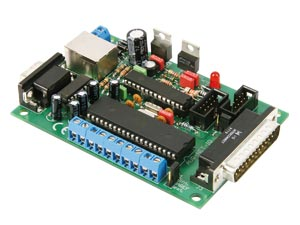
\includegraphics[width=10cm]{content/pictures/avr-net-io.jpg}
\caption{AVR-NET-IO - Pollin GmbH}
%http://www.pollin.de/shop/dt/MTQ5OTgxOTk-/Bausaetze_Module/Bausaetze/Bausatz_AVR_NET_IO.html
\label{fig:B3}
\end{figure}

\subsection{Technische Daten}
\begin{itemize}
  \item Betriebsspannung 9V
  \item Stromaufnahme ca. 190 mA
  \item 8 Digitale Ausgänge, 4 Digitale Eingänge
  \item 4 Analoge Eingänge
  \item ATmega32 Mikrocontroller
  \item integrierte ISP-Schnittstelle
\end{itemize}

\section{Mikrocontroller}
\subsection{ATmega32}

\subsection{ATmega644P}

\subsection{ATmega1284P}

\subsection{ENC28J60}

\section{Fuse Bits}
\label{chap:Fuse}

Die Fuse-Bits sind die Grundlegenden Einstellungen, mit denen ein
Mikrocontroller arbeitet. Sie müssen geändert werden, wenn ein anderer Taktgeber
gewünscht ist oder Schnittstellen de- oder aktiviert werden sollen.

\begin{myframe}
\textbf{Allgemeiner Hinweis:} Dieser Artikel kann die Recherche im Datenblatt
nicht ersetzen, besonders bei abweichendem Mikrocontroller sind die Fuse-Bits
oft anders gewählt. Mit dem Atmel Studio kann es vorkommen, dass man sich vom
Mikrocontroller aussperrt. Ein zurücksetzen der Fuse-Bits kann mit AVRDUDE
in diesem Fall versucht werden. Beschrieben wird dieser Vorgang im
Benutzerhandbuch \ref{Chapt:Einrichten}
\end{myframe}

In Tabelle ref{fuses-names} werden die einzelnen Fuse-Bits zusammen mit ihrer
Bedeutung und dem entsprechendem Byte aufgelistet. Der Schlussendliche Fuse Wert
setzt sich aus zwei Byte zusammen, wobei eine 1 eine deaktivierte Eigenschaft und
eine 0 aktiviert Eigenschaft bedeutet. Kleinere Mikrocontroller besitzen nur ein
High (H) und ein Low (L) Register, größere Mikrocontroller besitzen zusetzlich
noch ein Extended (E) Register.

\begin{table} [H]
\begin{tabular}{|l|l|l|} \hline
Fuse Name & Bedeutung & Bytes\\ \hline
BODLEVEL & Brown-out Detector trigger level & E-Fuse 0\&1\\ \hline
OCDEN & Aktiviert On-Chip Debuging & H-Fuse 7\\ \hline
JTAGEN & Aktiviert das \ac{JTAG} Interface & H-Fuse 6\\ \hline
SPIEN & Aktiviert das \ac{ISP} Interface & H-Fuse 5\\ \hline
WDTON & \ac{WDT} immer an & H-Fuse 4\\ \hline
EESAVE & Schützt den \acs{EEPROM} wärend des Lösch-Zyklus & H-Fuse 3\\ \hline
BOOTSZ & Boot Flash Sektor Größe & H-Fuse 1\&2\\ \hline
BOOTRST & Boot Reset Vektor & H-Fuse 0\\ \hline
CKDIV8 & Teilt den Takt der Uhr intern durch 8 & L-Fuse 8\\ \hline
CKOUT & Ausgabe des Takts der Uhr auf Port B1 & L-Fuse 7\\ \hline
SUT\_CKSEL & Wahl der Takt-Quelle & L-Fuse 0-6\\ \hline
\end{tabular}
\caption{Die Bedeutung der einzelnen Fuse-Bits (ATMega-664P)}
\label{fuses-names}
\end{table}

Wir benötigen für unseren ATMega-664P SPIEN, EESAVE und BOOTRST aktiviert im
High Register. Im Low Register muss alles deaktiviert werden, damit die Externe
Quarz-Kristall verwendet wird. Da das Brown-out Detector trigger level nicht
verwendet wird, kann in den Extended Register es ebenfalls alles deaktiviert
werden. Daraus resultiert die Bit Kombination in Tabelle \ref{fuses-result}.

\begin{table}[H]
\centering
\begin{tabular}{|l|l|l|} \hline
Fues Register & Binär & Hex\\ \hline
Extended-Fuse & 1111 1111 & FF\\ \hline
High-Fuse & 1101 0110 & D6\\ \hline
Low-Fuse & 1111 1111 & FF\\ \hline
\end{tabular}
\caption{Fuse Einstellungen (ATMega-664P)}
\label{fuses-result}
\end{table}

Im Atmel Studio können die Fuse Einstellungen ganz einfach im Device Programming
vorgenommen werden (Kapitel \ref{Chap:atmelStudio.Programming}). In Abbildung
\ref{fuses-graf} können sind die festgelegten Einstellungen eingetragen.

\begin{figure}[h]
\centering
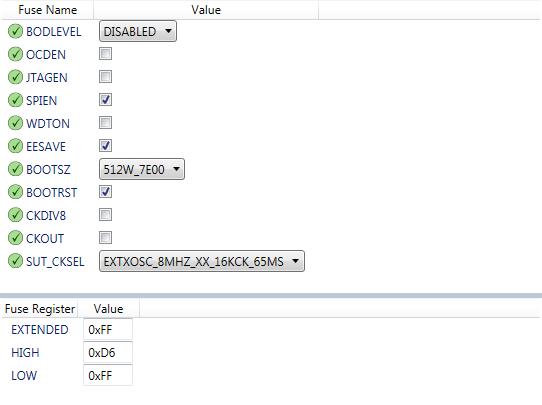
\includegraphics[width=13cm]{content/pictures/Fusebits/fusebits_atmelstudio.png}
\caption{Fuse-Bits im Atmel Studio (ATMega-664P)}
\label{fuses-graf}
\end{figure}


\chapter{Programmieren und Debuggen}

Um einen Mikrocontroller zu Programmieren oder zu Debuggen gibt es zwei
Interfaces, diese Werden hier einmal genauer Beleuchtet.

\section{ISP}

Ein \ac{ISP} fähiger Mikrocontroller kann direkt in der Schaltung Programmiert
werden, ohne entfernt zu werden. Programmieren kann man entweder mit dem
Programmer AVRISPmkII über die \acs{SPI} Schnittstelle oder mit dem  
AVRJTAGICEmkII. Der AVRJTAGICEmkII unterstützt zum Programmieren sowhol die
die \acs{SPI} als auch die \acs{JTAG} Schnittstelle.


\section{SPI}



\section{JTAG}


%Korrekturgelesen : Sophie Dietrich
\chapter{Recherche}

\section{Ethersex}

Auf der Projekt-Website (\url{http://ethersex.de}) bewirbt sich Ethersex als
\begin{quote} \textit{
		\enquote{[\ldots] eine Firmware mit Netzwerkunterstützung für 8-bit AVR
		Mikrocontroller, die durch eine Community entwickelt wird.  }
	}
	\cite{Ethersex}
\end{quote}

Ethersex unterstützt sowohl die von uns verwendeten ATmega Prozessoren, das
AVR-Net-IO Board und auch den verwendeten ENC28J60 Netzwerk Controller.
Durch einen ausführlichen Quick Start Guide
(\url{http://ethersex.de/index.php/Quick_Start_Guide/Preparation}) auf der
Projektseite ist es, auch für Anfänger in diesem Themengebiet, sehr einfach möglich, das Projekt lauffähig zu machen. 
Fast die gesamte Konfiguration kann über ein Menü vorgenommen werden. So muss nicht wie beim Radig Projekt zum
ändern der Mac Adresse in eine Headerdatei geschrieben werden. 

\begin{figure}[H]
	\centering
		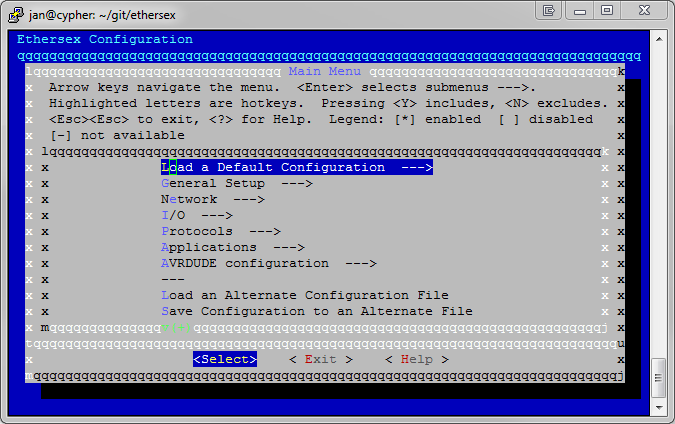
\includegraphics[width=13cm]{content/pictures/Recherche/Ethersex/Ehtersex1.png}
	\caption{Ethersex menuconfig}
	\label{Ethersex1}
\end{figure} 

Im Bild (Abb. \ref{Ethersex1}) sieht man den Startbildschirm des
Menüs, das über den Befehl \textrm{make menuconfig} erreicht werden kann.
Hier können verschiedene Einstellungen getroffen werden. Zum Beispiel, den
verwendeten Mikrocontroller, welche Mac Adresse der Netzwerk Controller
verwendet oder welche IP Adresse gewünscht ist.
Nachdem die Konfiguration abgeschlossen ist, kann das Hexfile mit dem
\textrm{make} Befehl erstellt werden. In der Abbildung \ref{Ethersex2} sieht man,
dass am Ende des \textrm{Make} Prozesses die aktuelle Größe des erstellten Binary Datei
angezeigt wird.

\begin{figure}[H]
	\centering
		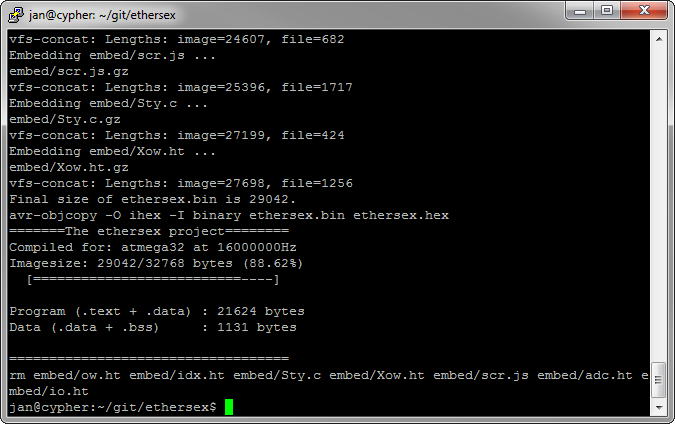
\includegraphics[width=13cm]{content/pictures/Recherche/Ethersex/Ethersex2.png}
	\caption{Ethersex make project}
	\label{Ethersex2}
\end{figure} 

Das Einbinden der Website beim Ethersex Projekt wird in der Anleitung
folgendermaßen beschrieben:

\begin{quote}
	\textit{
		\enquote{Falls die Option Supply Inline Files aktiviert ist, werden alle
		Dateien, die unter vfs/embed/ abgelegt sind, automatisch beim Erstellen des
		Images mit gzip gepackt und an das Ende der Firmware angehängt. Die
		Dateinamen bleiben dabei unverändert [\ldots]} }
	\cite[\url{http://www.ethersex.de/index.php/HTTPD_(Deutsch)}]{Ethersex}
\end{quote}

\section{Elektronik 2000}

Einen anderen Ansatz verfolgt das Projekt Elektronik 2000.
Hier wird nicht nur der Webserver geboten sondern eine erweiterte GUI, um das
Board zu programmieren. Dafür wird mit einem grafischem Designer eine Logik
entworfen und über einen ISP Programmer auf das Board gebracht.

\begin{quote}
	\textit{
		\enquote{Das E2000-NET-IO basiert auf dem AVR-NET-IO von Pollin. Durch die
		E2000-Firmware wird aus dem AVR-NET-IO von Pollin ein autak laufendes
		Logikmodul. Mit diesem Modul können über Netzwerk Schaltvorgänge ausgeführt
		werden. Außerdem sind Zeitgesteuerte Schaltvorgänge möglich.} }
	\cite{elektronik2000}
\end{quote}

Durch die Netzwerkanbindung des AVR-Net-IO kann dann die programmierte Logik von
außen überwacht und gesteuert werden. Dafür gibt es von den Entwicklern eine
bereitgestellte Android Applikation. Zusätzlich zu einem Projekt das mit dem
AVR-Net-IO arbeitet gibt es mittlerweile eine weitere Version, welche auch mit dem
Raspberry Pi zusammenarbeitet und die GPIO Pins des Pis nach außen steuerbar
macht.

\section{Ulrich Radig}

Ein weiteres Projekt für den AVR-Net-IO ist die AVR Webserver Software
(\url{http://www.ulrichradig.de/home/index.php/software/avr-webserver-software}).
Die Software ist ein Webserver für die Mikrocontroller der Baureihen ATmega 32,
64 und 128. Durch die Einfache Bindung der Dateien kann das Projekt
einfach an eigene Bedürfnisse angepasst werden. Dabei hat die Software noch
weiter Funktionalität:

\begin{itemize}
  \item \textbf{\ac{HTTP} Server} Webserver ohne Dateistruktur
  \item \textbf{Sendmail} Senden von E-Mails
  \item \textbf{Weather} Ermitteln von Wetterdaten
  \item \textbf{\ac{NTP}} Empfangen von Internetzeit
  \item \textbf{\ac{DNS}} Beantwortung von Anfragen zur
  Namensauflösung
  \item \textbf{\ac{USART}} eine Schnittstelle im Mikrocontroller zum
  Datenaustausch mit PC über die COM-Schnittstelle
  \item \textbf{\ac{Telnet}} zeichenorientierter
  Datenaustausch über eine TCP-Verbindung.
  \item \textbf{\ac{CMD}} Verwaltung der Telnet-Konsolenbefehle.
  \item \textbf{\ac{WOL}} Funktionalität um andere Geräte im Netzwerk
  durch bestimmte Datenpakete aufzuwecken.
\end{itemize}

%Korrekturgelesen: Ann-Sophie Dietrich
\chapter{Ausgewählte Lösung}

Neben den beiden anderen Projekten haben wir uns für das Projekt von Ulrich
Radig entschieden. Die Vorteile des Projektes gegenüber Ethersex oder Elektronik
2000 liegen darin, das die beiden Projekte zu speziell und umfangreich für unsere
Anforderungen sind. Da es zu unserem Aufgabengebiet gehörte eine für den
Benutzer möglichst umfangreiche Website zu erstellen kam uns die gut anpassbare
Lösung entgegen.

\section{Der Webserver}

Als Basis für unser Projekt haben wir die Firmware von Ulrich Radig verwendet.
Zusätzlich von der Ursprungsversion von Ulrich Radig gibt es noch eine etwas
vereinfachte Version von Günther Menke. Wir haben wir uns für die vereinfachte
Variante entschieden. Die Unterschiede zwischen beiden
Versionen belaufen sich auf das entfernte Kamera-Feature und auf
zusätzlichen Quellcode für einen alternativen Netzwerkcontroller.

\subsection{Änderungen}

Obwohl wir die bereits im Funktionsumfang vereinfachte Version
von Günther Menke verwenden, gab es trotzdem einiges an Funktionalität, welche wir
aus der ursprünglichen Version entfernt haben.
Das Problem lag darin, dass wir zum einen für die Dateien der Website möglichst
viel freien Speicherplatz benötigen, der von den entsprechenden Funktionen
belegt wurde. Zum anderen, dass die entfernten Funktionen nicht für unser
Projekt benötigt wurden. Schlussendlich wurden folgende Funktionalitäten aus der Version
von Günther Menke entfernt:

\begin{itemize}
  \item \textbf{(WOL) Wake on Lan} Funktionalität um andere Geräte im Netzwerk
  durch bestimmte Datenpakete aufzuwecken.
  \item \textbf{Sendmail} Senden von E-Mails
  \item \textbf{Weather} Ermitteln von Wetterdaten
  \item \textbf{(NTP) Network Time Protocol} Empfangen von Internetzeit
  \item \textbf{(DNS) Domain Name System} Beantwortung von Anfragen zur
  Namensauflösung
  \item \textbf{(USART) Universal Synchronous and Asynchronous Serial Receiver and
  Transmitter} eine Schnittstelle im Mikrocontroller zum Datenaustausch mit PC über die COM-Schnittstelle
  \item \textbf{(Telnet) Telecommunication Network} zeichenorientierter
  Datenaustausch über eine TCP-Verbindung.
  \item \textbf{(CMD) Command Control} Verwaltung der Telnet-Konsolenbefehle.
\end{itemize}

\subsection{Einbindung der Website}

Die Website, welche hauptsächlich aus verschiedenen .html und .js Dateien
besteht, ist mangels Dateisystem für unsere Firmware nicht verwendbar. Die
gesamten Dateien müssen in einer C-Headerdatei gebunden werden.
Das Erstellen der Headerdatei erfolgt über das beim Projekt beigelegte
\ac{HHC} Werkzeug. Eine Beispiel zum Erstellen der \textrm{webpage.h} 
Datei und eine Erklärung des \ac{HHC} gibt es im Kapitel Werkzeuge
\ref{chap:hintergrund.HHC}. Eine Anleitung zur Ausführung des \ac{HHC} gibt es im
Benutzerhandbuch \ref{chap:benutzerhandbuch.HHC}.
Abschließend ist noch zu erwähnen, dass die \textrm{webpage.h} nicht für manuelle
Bearbeitung gedacht ist. Dies geschieht ausschließlich über die Quell-Dateien
und anschließendem umwandeln mit dem \ac{HHC}.

\section{Die Website}

Der Aufbau der Webseite ist in mehrere Dateien aufgeteilt. So haben wir mehrere
.js und .css Dateien. In der index.html wird alles nur zusammengetragen.

\subsection{HTML und CSS}
Es gibt nur eine html Seite in der alle anderen Dateien aufgerufen werden und zur
Hauptseite wird: Die index.html\newline
Die CSS-Elemnte sind in mehrere Dateien aufgesplittet. So kann die input.css
gegen eine andere input.css ausgetauscht werden. Die input.css ist die Datei für
das Desgin mit den Farben, Formen, usw.\newline
Eine weitere .css Datei sollte nicht ausgetauscht werden (board.css).

\subsubsection{board.css}
Diese Datei behandelt alle Definitionen über die Platine in dem "`Status
Tab"' der Webseite. Diese Definitionen werden in der index.html in einem 'div-Salat' zu einer
Platine, die auch klickbar ist, zusammengebaut. Löschen eines Divs verursacht
Darstellungsfehler, sowie keine weitere Anzeige der grafischen Platine.

\subsection{JavaScript}
\subsubsection{Generell}
In \textrm{rest.js} und \textrm{favorite.js} werden die einzelnen Pins über eine
ID unterschieden. Diese ID wird vor allem als Parameter für diverse Funktionen
wie \textrm{getValu(id)} verwendet. Die ID setzt sich immer aus dem Buchstaben des
Ports, sowie aus der Nummer des Pins zusammen. Mögliche IDs sind folglich [A0
bis A7], [C0 bis C7] und [D0 bis D7].

\subsubsection{rest.js}
Die \textrm{rest.js} beinhaltet den gesamten Code zum Abrufen von Daten beim
Server.

Hierbei bieten die Funktionen \textrm{loadUrl(\ldots)} und
\textrm{loadUrlAsync(\ldots)} den Kern der Serverkommunikation. Mit ihnen können
beliebige URLs geladen werden, \textrm{loadUrlAsync(\ldots)} bietet zusätzlich
die Möglichkeit POST-Parameter zu übergeben. Der grundlegende Unterschied
zwischen diesen beiden Methoden ist, dass \textrm{loadUrl(\ldots)} den
Programmablauf blockiert, bis die Daten vollständig geladen sind, wohingegen
\textrm{loadUrlAsyn(\ldots)} die Daten parallel im Hintergrund lädt. Sobald alle
Daten erfolgreich geladen sind, wird die Funktion aufgerufen, die
\textrm{loadUrlAsync(\ldots)} als Parameter übergeben wurde. Weitere
Informationen, vor allem zur Parametisierung der Funktionen, sind der
Sourcecode-Dokumentation zu entnehmen.\\
\\
In der Funktion \textrm{initRest()} wird zum ersten Mal die Funktion
\textrm{startNewRefreshTask()} aufgerufen. Diese ruft die Funktion
\textrm{refreshValues()} auf, welche sich selbst rekursiv immer wieder nach
einer gewissen Pause (der Polling-Frequenz, welche in den Einstellungen
festgelegt werden kann) aufruft. Die Polling-Frequenz wird in dem Attribut
\textrm{pollingFreq} gespeichert. Der so erzeugte Refersh-Task, der
vollautomatisch die Werte aktualisiert, kann über \textrm{cancelRefreshTask()}
wieder gestoppt werden. Die Werte werden danach natürlich nicht mehr
aktualisiert, bis mit \textrm{startNewRefreshTask()} ein neuer Task gestartet
wird. Nach jedem Aktualisieren der Werte wird die Funktion aufgerufen, die in
dem Attribut \textrm{onValuesChanged} gespeichert wird. In unserer
Implementierung ist diese Funkion in der \textrm{ui.js} implementiert und
organisiert die Aktualisierung der Oberfläche, damit die aktuellen Werte
dargestellt werden. Der Wert des Attributes \textrm{onValuesChanged} kann mit
der Funktion \textrm{setOnValuesChanged(\ldots)} manipuliert werden. Die zuletzt
empfangenen Werte werden in \textrm{cachedValues} gespeichert und sind über
diverse Getter wie \textrm{getValue(id)} verfügbar.

Das Stoppen eines bestehenden Tasks wird realisiert, indem das Attribut
\textrm{taskIdCounter} inkrementiert wird. \textrm{refreshValues()} überprüft am
Anfang ob der aktuelle Wert von \textrm{taskIdCounter} mit dem Wert
übereinstimmt, mit der der aktuell ausgeführte Task gestartet wurde. Ist dies
nicht der Fall, weil der Task beendet oder ein neuer gestartet wurde, beendet
sich der Task automatisch selbst, indem die Funktion \textrm{refreshValues()}
nicht erneut rekursiv aufgerufen wird.\\
\\
In der Funktion \textrm{initRest()} werden einmalig die REST-URLs
\textrm{/rest/info} und \textrm{/rest/pininfo} geladen. Diese beinhalten nur
statische Informationen, welche sich nie ändern. Die empfangenen JSON-Strukturen
werden in ein javaScript Objekt geparst und in \textrm{cachedInfo} und
\textrm{cachedPinInfo} gespeichert. Der Inhalt dieser Objekte wird über
die Getter \textrm{getInfo()} und \textrm{getPinInfo()} zur Verfügung gestellt.
Für \textrm{cachedPinInfo} sind zudem Getter wie
\textrm{getDefaultDescription(id))} vorhanden.


\subsubsection{favorites.js}

In der favorites.js wird eine Liste alles Pins angelegt. Hier kann der Nutzer für jeden Pin eine
Beschreibung, sowie eine Funktion und ob dieser Pin als Favorit markiert werden soll, 
hinterlegen. Diese Liste wird dann in eine lokale Datenbank abgespeichert und bei Neustart aus dieser ausgelesen. 
Zusätlich kann diese durch Import und Export Funktionen als reiner Fließtext ausgegeben und auf anderen Rechnern 
eingefügt werden, damit die Daten dort ebenfalls exisiteren.\\
Ursprünglich sollte favorites.js nur eine Liste der als Favorit markierte Pins speichern, 
was jedoch nach einigen Überlegungen zu einer Liste aller Pins umgeändert wurde. Der Name 
"`favorite.js"' wurde jedoch beibehalten.

\subsubsection{db.js}
Die \textrm{db.js} besteht aus 2 Funktionen: 

\textrm{getDb(key, defaultValue)} liefert den gespeicherten Wert für den
gegebenen \textrm{key}, welcher immer eine Zahl oder ein String sein sollte. Ist
kein Wert mit dem gegebenen Key vorhanden, wird der
übergebene \textrm{defaultValue} zurückgegeben.

\textrm{putDb(key, value)} speichert das gegebenen \textrm{value} unter dem
gegebenen \textrm{key} ab. Wird jetzt \textrm{getDb(key, defaultValue)} mit dem
gleichen \textrm{key} aufgerufen, wird der zuvor abgespeicherte Wert
zurückgegeben.

Alle Mit \textrm{db.js} gespeicherten Werte sind auch nach einem Neuladen der
Seite weiterhin verfügbar, solange nicht die IP-Adresse des Pollin Net-IO Boards
verändert wird. Die verwendeten Keys müssen natürlich eindeutig sein.

\subsubsection{ui.js}
Die \textrm{ui.js} beinhaltet den gesamten Code für das dynamische Gestalten der
Webseite\newline
Ein der wichtigsten Funktionen, die generell verwendet wird, ist die
\textrm{getEl(id)}.
Diese Funktion verkürzt die Standardfunktion von JavaScript
\textrm{getElementById(id)}, um den Sourcecode zu kürzer zu halten,
um den daraus resultierenden Speicherbedarf der Webseite zu
minimieren.\newline

\textrm{initUi()} sollte nur einmal beim Seitenaufruf geladen werden und
initialisiert die Bneutzerschnittstellen. \textrm{setMain(div)} setzt die
Hauptkoponenten von dem Frame 'div'.\\
\textrm{addClass(clazz, item)} fügt eine CSS Klasse zu dem gegebenen Item hinzu,
während die \textrm{removeClass(clazz, item)} die CSS Klasse von dem Item wieder
löscht.\\
\textrm{getHighlightElem(id)} makiert die digitalen Pins, oder makiert die
Checkboxen der analogen Pins.
Folgende Funtkionen generieren die dynamische Sidebar: \textrm{setSidebarId(id)}
listet alle Informationen über die Pins in der Sidebar auf. Die
\textrm{updateSidebarValues()} hält die Werte der einzelnen Pins auf den
aktuellsten Stand.\\
Die Favoriten Tabelle wird mittels der Funktion \textrm{updateFavoritesTable()}
erneuert und mit \textrm{updateFavoritesTableValues()} werden die Pininformationen 
der Favoriten auf den aktuellsten Stand gebracht. Ändern sich die
Favoriten wird \textrm{onFavoritesChanged()} aufgerufen.\\
\textrm{text}\\
Das seperat aufpoppende Fenster um die Pins / Ports besser zu konfigurieren wird
mit \textrm{startConfigurePin(id)}. Beim Aufruf wird die ID des Pins benötigt.
In der Funktion werden die restlichen Informationen zu dem Pin abegrufen und
eingetragen. In dem Fenster sind die Buttons 'OK' und 'zurücksetzen', die dann
beim bestätigen \textrm{endConfigurePin(reset)} aufruft. reset ist der Flag
zum zurücksetzen des Pins. Ist er auf true, wird der Pin zurückgesetzt, sollte
er auf false sein, werden die neuen Konfigurationen zum Pin abgespeichert.\\
Um die index.html nicht noch mit weiteren vielen div-Elemnten zu
überfüllen, werden die gleichen div-Elemente mit \textrm{write(count, string,
ids)} generiert. Diese Funktion wird in folgenden verwendet:
\textrm{writePinCheck(ids)}, \textrm {writePinCheckMinus(count)},
\textrm{writePinCheckPlus(count)}, \textrm{writePinCheckNone(count)},
\textrm{writePinMinusBox(count)}, \textrm{writePinCheckAnalog(ids)} und
\textrm{writeAnalogBox(ids)}.




\chapter{Technischer Hintergrund}

\section{Vorgeschlagene Lösung}

\subsection{Kommunikation im Projekt Radig}
Im Projekt Radig ist keine echte Kommunikation zwischen dem Client und dem Server 
vorhanden. 

Die auf der Webseite dargestellten Werte werden vor dem senden der HTML-Seite 
im HTML-Code eingefügt indem Platzhalter im Format "`\%PORTA0"' ersetzt und so statisch auf 
der Webseite dargestellt werden. Das Manipulieren der Pins findet über ein HTML-Formular 
statt. Alle manipulierbaren Pins sind als Input vom Typ Checkbox dargestellt. Diese lassen 
sich frei manipulieren und erst beim Betätigen des "Senden"-Buttons werden die 
Informationen per POST-Event an den Server gesendet und so die Seite neu aufgerufen. Der 
Server filtert die POST Informationen aus dem HTTP-Header und manipuliert die Pins gemäß 
den Anweisungen. Beim senden des angeforderten HTML-Dokumentes werden die neuen Werte in 
den HTML-Code eingefügt, und so die neuen Werte auf der Webseite angezeigt.

Das große Problem bei dieser technisch einfachen Lösung ist, das geänderte Werte erst beim 
nächsten neu laden der Webseite angezeigt werden. Ändert sich ein Pin während die Webseite 
dargestellt wird bekommt der Nutzer dies nicht mit. Zudem wird bei jedem Manipulieren 
eines Pins die gesamte Seite neu geladen und so Unmengen an unnötigen Daten übertragen. 
Auch zum darstellen der aktuellen Werte muss die ganze Seite neu vom Server angefordert 
werden.

\subsection{Erster Ansatz}
Die Kommunikation zwischen Server und Client sollte mit Hilfe einer REST-Schnittstelle 
stattfinden, die im Hintergrund über Javascript angesprochen werden kann. 

Eine REST-Schnittstelle besteht aus einer oder mehreren virtuellen URLs. Beim Aufruf einer 
solchen URL liefert der Server kein Dokument das gespeichert ist, sondern erzeugt 
dynamisch eine Antwort mit den benötigten Informationen und sendet diese als Antwort 
zurück. Der Server kann beim Aufruf einer URL auch eine Aktion ausführen.

Vorteile der REST-Schnittstelle ist die simple Implementierung, sowohl auf dem Client mit 
JavaScript als auch auf dem Server. Die Inhalte werden mit JSON formatiert, welches einen 
technisches Standart darstellt und sich in JavaScript direkt in ein Objekt umwandeln 
lässt. Auf dem Server ist es einfach mit einem Stringformat immer gleiche JSON Strukturen 
zu erstellen und nur aktuelle Werte einzufügen. Die REST-Schnittstelle lässt sich leicht 
um weitere, neue Funktionalitäten erweitern, indem neue virtuelle URLs erstellt werden die 
vom Client ansprechbar sind.

Die Anforderungen an eine Lösung in diesem Projekt waren vor allem eine möglichst kompakte 
Schnittstelle zu schaffen die wenig Bandbreite verbraucht um eine hohe 
Übertragungsgeschwindigkeit zu ermöglichen trotz des schwachen Servers. Ein besonderes 
Augenmerk war auf die Übertragung der Messwerte zu legen, da diese nicht wie andere 
statische Informationen nur einmalig übertragen werden sondern kontinuierlich erneuert 
werden müssen. Die Schnittstelle sollte gut skalierbar sein. Würde später ein Port für
eine andere Aufgabe zu verwendet werden muss dieser Port ohne Aufwand aus der 
REST-Schnittstelle ausgeschlossen werden können, damit er von außen nicht manipulierbar 
ist und so interne Abläufe auf der Platine nicht gestört werden.

Nach den Anforderungen muss die Schnittstelle folgende Aufgaben ermöglichen:
\begin{itemize}
\item Abfragen der aktuellen Werte aller verwendbaren Pins
\item Abfragen der Konfiguration eines Pins (Eingang oder Ausgang)
\item Abfragen von Allgemeinen Informationen des Boards (IP, Standart-IP, Mac-Adresse,
	Serverversion)
\item Manipulieren aller als Ausgänge geschaltener Pins
\item Manipulieren der Konfiguration eines Pins (als Eingang oder Ausgang setzen)
\item Manipulieren von Servereinstellungen (z.B. IP-Adresse);
\end{itemize}

%\begin{itemize}
%	\item Aufbau als REST-Schnittstelle
%	\begin{itemize}
%		\item Simpel implementierbar
%		\item Technischer Standart
%		\item Fertige Mechaniken in JavaScript
%		\item Leicht erweiterbar um neue Funktionalitäten
%	\end{itemize}
%	\item Anforderungen an eine Lösung:
%	\begin{itemize}
%		\item Möglichst kompakt, wenig Bandbreite soll verbraucht werden
%		\item Messwerte müssen besonders effizient übertragen werden
%		\item Skalierbar - Egal ob ein oder 20 Ports verwendet werden
%		\item Neben Abfragen der Messwerte auch manipulieren der IP, des DDR und der 
%			  Ausgänge
%		\item JSON-Encodiert, direkt in JavaScript Objekt überführbar
%	\end{itemize}
%\end{itemize}

%-----------------------------------------------------------------------------------------
\subsection{Polling oder Pushing}
Die aktuellen Werte der Pins müssen bei jeder Änderung vom Server zum Client übertragen 
werden, damit diese auf der Webseite immer korrekt dargestellt werden. Hierfür stehen zwei 
verschiedene Konzepte zur Verfügung wie die Übertragung der Daten initialisiert werden.

\subsubsection{Polling}
Bei Polling werden vom Client kontinuierlich die Werte erneut angefordert, indem dieser 
die entsprechende virtuell URL des Servers aufruft. Dies führt dazu, dass viele unnötige 
Date übertragen werden, da sich eventuell nicht bei jedem erneuten anfordern der Werte 
diese auch tatsächlich verändert haben und so die gleichen Datensätze oft mehrmals 
angefordert werden.

Im vergleich zu der Radig-Lösung bietet Polling den Vorteil das die Werte kontinuierlich 
nach geladen und so immer korrekt dargestellt werden während die Webseite dargestellt 
wird. Auch das gesendete Datenvolumen wird dahingehend minimiert, das nur die Nutzdaten 
übertragen werden und nicht der gesamte HTML-Code der Webseite. Polling ist technisch sehr 
einfach zu realisieren, da die Abfrage der Daten einfach zyklisch wiederholt werden.

\subsubsection{Pushing}
Bei Pushing wird im Gegensatz zu Polling der Daten nicht vom Client initialisiert sondern 
vom Server. Der Server weiß wann sich die Werte geändert haben und kann dem Client bei 
jeder Änderung gezielt die neuen Daten Übermitteln. Das Übertragen der Daten könnte z.B. 
durch einen Interrupt ausgelöst werden.

Im direkten vergleich zu Polling bietet Pushing verschiedene Vorteile. So wird nicht nur 
das Volumen der übertragenen Daten reduziert indem keine unnötigen Abfragen stattfinden,
sondern die neuen Werte gelangen auch genau dann zum Client wenn die Änderung tatsächlich 
stattgefunden hat, was dazu führt das die Webseite schneller auf Änderungen reagiert.

Die technische Umsetzung von Pushing ist mit diversen Problemen verbunden. Die typische 
Verbindungsaufbaurichtung ist bei Webanwendungen und Webseiten immer vom Client zum 
Server. Anders als bei Polling müssen bei Pushing Daten vom Server zum Client gelangen. 
Hierfür muss eine Verbindung vom Server zum Client aufgebaut werden. Dies ist technisch 
aber nicht möglich, da der Browser bzw. JavaScript keine Möglichkeit haben einen Port des 
Clientsystems zu öffnen und auf eingehende Verbindungen des Servers zu antworten. 

Das Problem lässt sich durch die Benutzung von HTML5 Server-Sent Events umgehen. Hierbei 
frägt der Client eine virtuelle URL des Servers ab, ähnlich einer REST-Schnittstelle. Der 
Server überträgt jedoch nicht sofort Daten, sondern schreibt erst bei einem Event (z.B. 
die Änderung eines Pins) in den geöffneten Stream und pusht so die Daten zum Client. 
Dieser überwacht den Stream mit Hilfe von JavaScript un empfängt so die neuen Werte und 
kann sie auf der Webseite anzeigen.

Dieses System ist auf dem Pollin Net-IO Board aber nur schwer umzusetzen da mehrere 
Verbindungen verwaltet werden müssen. So ist immer mindestens eine Server-Sent Event 
Verbindung offen, parallel könnte aber ein Client andere Daten vom Server anfordern. Für 
das Verwalten mehrerer Verbindungen sind aber viele Resourcen nötig, da für jede 
Verbindung auch Daten im RAM hinterlegt werden müssen. Außerdem st in vielen Situationen 
ein simples Multitasking nötig, das so auf einem ATmega CPU nicht vorhanden ist. Das Radig 
Projekt setzt aus diesen Gründen auf HTTP 1.0 bei dem für jede Anfrage eine Verbindung 
geöffnet und nach erfolgreichem Übertragen der Daten wieder geschlossen wird. So ist auch 
die Kommunikation mit mehreren Clients problemlos möglich.

Um HTML5 Server-Sent Events auf dem Pollin Net-IO Board zu implementieren würde es als 
einen tendenziell größeren CPU erfordern mit dem auch Multitasking möglich ist sowohl auch 
eine grundlegende Umgestaltung des Radig-Projektes um mehrere HTTP Verbindungen parallel 
zu ermöglichen.

\subsubsection{Entscheidung}
Da die technische Umsetzung vom Pushing nur schwer möglich ist werden wir auf Polling 
setzen.

TODO: Hier noch Argumentation mit Übertragungszeit und Screenshot aus Chrome Network Log


%\begin{itemize}
%	\item Daten können entweder per Polling vom Client (Webseite abgefragt werden) oder
%		  vom Server bei einem Event (Änderung eines Eingangs) per Push geschickt werden	  
%	\item Pro/Contra Push
%	\begin{itemize}
%		\item Pro: Daten werden nur übertragen wenn es wirklich nötig ist, kein unnötiger 
%			  Datenverkehr
%		\item Pro: Leistung bleibt auch mit mehreren Clients eher konstant 
%			  (Genau Begründung ausarbeiten!)
%		\item Pro: Board wird entlastet, kein DOS, mehrere Clients können Webseite 
%		      trotzdem problemlos aufbauen 
%	\end{itemize}
%	\item Pro/Contra Polling
%	\begin{itemize}
%		\item Pro: Leichter zu implementieren - normale Dateiabfrage
%		\item Contra: Es werden viele unnötige Daten übertragen
%		\item Contra: Leistung nimmt mit steigender Anzahl von Clients ab
%		\item Pro: Im Prinzip nicht langsamer als Push: Limitierende Komponente ist die 
%			  Übertragungszeit! (Hier Bild von Chrome Netzwerkvehrkehr) 
%	\end{itemize}
%	
%	\item Push bessere Lösung
%	\item Umsetzung aber nicht möglich
%	\item Server kann keine Verbindung zu Client aufbauen
%	\begin{itemize}
%		\item Javascript kann keinen Serverport öffnen
%		\item Client hat keine öffentliche IP
%	\end{itemize}
%	\item Technische Lösung: HTML 5 Server Sent Events
%	\begin{itemize}
%		\item Technischer Standart, Eingeführt mit HTML 5
%		\item Client ruft virtuelle URL auf, ähnlich REST
%		\item So wird ein Stream geöffnet
%		\item Bei einem Event schreibt der Server die Informationen in den Stream
%		\item Client benutzt Javascript API um die jeweiligen Informationen zu lesen
%	\end{itemize}
%	\item Mit ATmega CPU und Radig Projrkt als Vorlage nicht lösbar
%	\begin{itemize}
%		\item Radig kann nur eine Verbindung handeln. Aufbau - Übertragung - Abbau für 
%			  jede Datei
%		\item HTTP 1.0
%		\item Aufruf einer HTML5 Server Sent Event URL würde dazu führen das der Server 
%			  blockiert ist
%		\item Gesamte Struktur auf nur eine Verbindung ausgelegt
%		\item Bei Umschreiben (sehr tiefer Eingriff!) stößt die CPU schnell an Grenzen
%		\item Multitasking nötig, Stack für jede Verbindung führt zu RAM Problemen
%		\item Sprengt vermutlich zeitlichen Rahmen
%	\end{itemize}
%	\item Daraus resutltiert die Verwendung von Polling
%	\item Da Polling nicht langsamer ist, gibt es keine Nachteile bei Frequenzen von ca. 
%		  200ms (auch bei zB. 3 Clients)
%\end{itemize}

%-----------------------------------------------------------------------------------------
\subsection{Aufbau der REST-Schnittstelle}

\begin{itemize}
	\item 6 URLS
	\item ..........Hier Zitat aus Präsentation, aber noch anpassen!
\end{itemize}
	
%-----------------------------------------------------------------------------------------
\subsection{Implementierung der REST-Schnitstelle auf dem Server}

Für die Restschnittstelle wurde Weitestgehend der Bestehende Quellcode von Radig
verwendet. Zum auslesen ob ein Pin gesetzt ist sind Platzhalter vorgesehen.
Das Schema für so einen Platzhalter ist \textrm{\%PINXY} und setzt sich zusammen aus dem
Aufruf \textrm{\%PIN}, dem anzusprechendem Port X = [A,C oder D] und dem Pin Y = [0-7] (z.B.
\textrm{\%PINC1 } ). Mit diesem Platzhalter kann der direkte Pin Ausgelesen
(Hier Port C und Pin 1) und an eine beliebige Stelle im Quellcode platziert werden. Neu
hinzugekommen ist das Ausgeben der Information ob der Konkrete Pin über das
DDRegister als Ein- oder Ausgang definiert ist. Das Schema ist für diesen
Platzhalter ist \textrm{\%DDRXY} und setzt sich zusammen aus dem Aufruf \textrm{\%DDR}, dem
anzusprechendem Port X = [A,C oder D] und dem Pin Y = [0-7] (z.B.
\textrm{\%DDRD1} ). \\
\\
Damit das System für uns möglichst flexibel Arbeitet, haben wir uns dafür
entschieden, diese Dynamischen Angaben in eine Separate Datei auszulagern und
über die REST Schnittstelle abzufragen. Konkreter liegt in dem /Rest
Verzeichnis eine \textrm{values} Datei die die Platzhalter enthält. Zusätzlich
gibt es noch eine \textrm{info} und \textrm{pininfo} Datei, die statische
Informationen zu den Pins und Ports Enthält. \\
\\
Das setzen der Ausgänge wird über einen HTTP-Post Aufruf getätigt. So können die
Pins des entsprechenden Ports gesetzt oder umgeschaltet werden. Die
Informationen, die zum setzen eines Ports benötigt werden setzen sich zusammen
aus einem \textrm{SET} Befehl und dem Aufruf PORTXYZ zum setzen oder dem
\textrm{SET} Befehl und dem Aufruf OUTXYZ. X steht für den anzusprechendem Port
X = [A,C oder D]. Y und Z Stehen für die Einstellung der Pins in hexadezimaler
Schreibweise (00-FF) Abschließend muss das Ende der Schaltanweisung mit
\textrm{SUB} gekennzeichnet werden, da der Webserver auf diese Steuerzeichen
prüft. Ein Beispiel Post zum setzen der Pins C0-C3 auf Ein, der Pins C4-C7 auf
Aus, dem umschalten der Pins D0-D3 als Ausgang und der Pins D4-D7 als Eingang
sieht folgendermaßen aus:
\\

\framebox{SET=PORTC0F\&SET=OUTD0F\&SUB=Senden} 
%\begin{itemize}
%	\item Benutzung der Struktur von Radig
%	\item Die Eingägne werden durch Platzhalter (z.B. \%PortC1 ) angegeben. Beim
%			übertragen des Dokuments werden die Platzhalter ersetzt durch passende Werte
%	\item in /rest liegen Dateien values (mit Platzhaltern), pininfo und info
	% (jeweils als
%	      statisches Dokument)
%	\item Dateien können von ausßen normal aufgerufen werden und werden ggfs. mit
	% realen
%	      Informationen aufgefüllt
%	\item Vorteil: Test außerhalb der Platine möglich, da Werte als String
	% gekennzeichnet
%	      sind in JSON, Pins haben dann den Wert \%PortXY anstatt 0 oder 1
%	\item TODO: Wie werden die set URLs implementiert?
%	\item Die Ausgänge werden über die Post übertragung gesetzt.
%\end{itemize}

%-----------------------------------------------------------------------------------------
\subsection{Implementierung der REST-Schnitstelle auf dem Client}

\begin{itemize}
	\item Aufruf der URLs im Hintergrund mit Ajax
	\item info und pininfo werden zu Beginn einmalig aufgerufen (synchron um zu 
	      gewährleisten das die Daten zur Verfügung stehen für andere Initialisierungen)
	\item values wird mit setTimeout(...) zyklisch assynchron aufgerufen
	\item synchrones aufrufen von values führt dazu, das sich die Webseite aufhängt, da
	      der (Single-)JavaScript Thread mit dem laden der Daten beschäftigt ist und nicht
	      für andere Aufgaben zur Verfügung steht. Bei einem assynchronen Aufruf werden 
	      die Daten von einem anderen Thread im Hintergrund geladen
	\item JSON-Text wird mit JSON.parse(...) in ein Objekt transformiert
	\item Informationen werden über entsprechende getter zur Verfügung gestellt
	\item Funktion onValueChanged wird jedes mal aufgerufen wenn neue Daten zur 
	      Verfügung stehen
	\item onError wird aufgerufen wenn ein Fehler in der Kommunikation aufgetreten ist
	\item Über setter werden die entsprechenden URLs assynchron aufgerufen und so die 
	      Daten an den Server übermittelt
\end{itemize}

\section{Werkzeuge}

\subsection{Das Atmel Studio}

\subsubsection{Device Programming}

Eine Kernkomponente beim Atmel Studio ist das Device Programming Fenster.
Erreicht werden kann es über "`Tools $\to$  Device Programming"'.
Hier kann die Aktuelle Verbindung mit dem Microcotroller bestimmt werden, es
können die Fuse Bit Einstellung geändert werden oder einzelne Hex
Dateien auf den Mikrocontroller aufgespielt werden.



Übersicht k Gerät Auswählen
Contoller Auswählen
Spannung und Signatur
Fuse Bits
Hexfile Flashen

\begin{figure}[h]
\centering
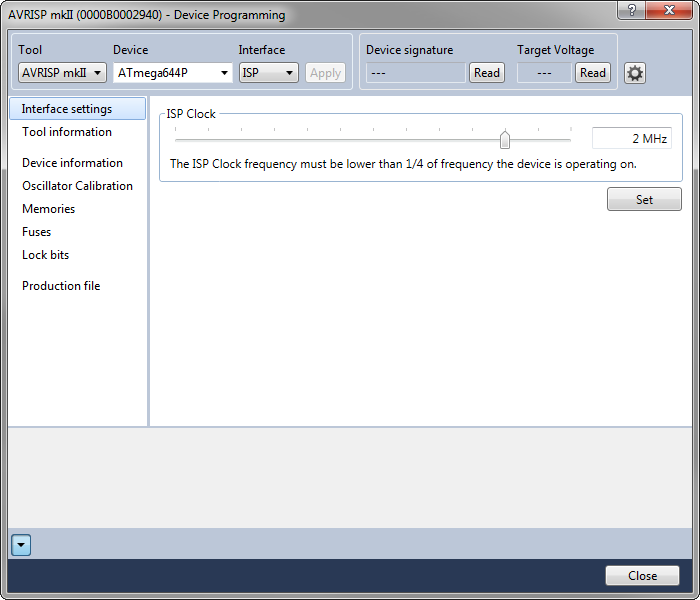
\includegraphics[width=13cm]{content/pictures/Anleitung/neuerProzessor/AnleitungNeuerProzessor1.png}
\caption{DeviceProgramming}
\label{fig:B3}
\end{figure}

\subsubsection{Projekt Einstellungen}

Taktfrequenz
Programmer
Empfolene Tool Settings

\subsection{AVRDUDE}

Avrdude ist ein Alternatives Werkzeug zum Bearbeiten von Mikrocontrollern. Es
ist im Gegensatz zum Atmel Studio lediglich ein Konsolen Werkzeug ohne
grafische Oberfläche. Mit Avrdude können unter anderem die Fusebits von einem
Mikrocontroller gelesen und gesetzt werden. Weiter ist es möglich eine Sicherung
von dem Aktuellen stand des Mikrocontrollers herzustellen oder ein Hex Datei auf
den Mikrocontroller aufzuspielen. Avrdude unterstützt eine Reihe von ISP Geräten
unter anderem auch den von uns verwendeten Atmel AVRISPmkII. Der Einsatz von
Avrdude war notwendig, da die Fusebits von einem Neuen Microcontroller
Standartmäßig auf den internen Quarz-Kristall gesetzt sind und nicht auf den
Externen Kristall des AVR-NET-IO Boards.
Eine genaue Anleitung gibt es im Kapitel \ref{chap:Benutzerhandbuch}
Benutzerhandbuch.

\subsection{HTML Header Compiler}
\label{chap:hintergrund.HHC}

Zum automatischen umwandeln der Quell-Dateien (html, js, png etc\ldots) haben
wir einen speziellen HTML Header Compiler entwickelt der die Website in eine
für den Webserver verständliche Headerdatei umwandelt. Der Compiler durchsucht
den Eingabe Ordner und sammelt die darin enthaltenen Dateien. Daraus entsteht
dann die für das Projekt benötigte Header Datei, bestehend einem Array von
Buchstaben für jede Datei. Der \ac{HHC} ist den Projektdateien, mit denen diese
Dokumentation ausgeliefert wurde beigelegt, kann aber auch zusammen mit dem
Projekt auf Github \url{https://github.com/doofmars/Embedded-Webserver}
bezogen werden.\\

Eine Beispiel Umwandlung: 

\begin{figure}[H]
\lstinputlisting[language=HTML]{content/code/index.html}
\caption{index.htm}
\label{HHC.input}
\end{figure}

Das eingegebene Verzeichnis, welches die \textrm{index.html} Datei enthält wird
eingelesen und in die folgende Headerdatei umgewandelt.
Abbildung \ref{HHC.input} zeigt eine simple "`Hallo Welt"' Website, die keine
weitere Funktion besitzt. Nachdem die Website mit dem HTML-Header-Compiler
umgewandelt wurde, entsteht die Headerdatei aus Abbildung \ref{HHC.output}. Gut
zu erkenne ist das Array aus Buchstaben in hexadezimaler Schreibweise welches die
index.html Datei widerspiegelt.
Am Ende der Headerdatei ist ein weiteres Array, bestehend aus Schlüssel-Wert
paaren für den Webserver. Hier wird hinterlegt welche Dateien vorhanden sind.
Der letzte Eintrag in diesem Array signalisiert das Ende der Suche und ist die
Bedingung für den Webserver um zur Standardausgabe zu wechseln. Bsp: Eine HTML
Datei wird angefordert die nicht existent ist, resultiert in der Ausgabe von
index.html.

\begin{figure}[H]
\lstinputlisting[language=C]{content/code/webpage.h}
\caption{webpage.h}
\label{HHC.output}
\end{figure}

Anzumerken ist das Standardmäßig der HTML Header Compiler die eingegebenen HTML
und JS Dateien optimiert in die Headerdatei speichert. Dazu wird die
Formatierung für den Zeilenvorschub, Tabulator oder Wagenrücklauf entfernt.
Falls dies für die Entwicklung nicht gewünscht ist, kann man diese Funktion
durch den Parameter \textrm{-n oder -newline} deaktivieren.
Außerdem ist die entstandene Headerdatei nicht zur Bearbeitung gedacht. Die
Bearbeitung erfolgt ausschließlich im Quelltext (z.B. der index.html). Analog
kann man dazu einen beliebigen Compiler einer herkömmlichen Programmiersprache sehen. Dieser
erzeugt aus dem Quelltext eine Binärdatei, diese ist nicht unbedingt
für Menschen lesbar. Bei Änderungen wird der Quelltext angepasst und neu
Compiliert. Da die Headerdatei folglich nicht bearbeitet werden muss haben wir
uns für eine Ausgabe als Array aus Buchstaben in hexadezimaler Schreibweise
entschieden, da es eine einfachere Programmatische Strukturierung erlaubt.

\subsection{AVRISPmkII}


\subsection{AVRJTAGICEmkII}



%Korrekturgelesen: Ann-Sophie Dietrich
\chapter{Benutzerhandbuch} 
\label{chap:Benutzerhandbuch}

\section{Einen Mikrocontroller austauschen}
Für unser Projekt sollen alle notwendigen Programmbestandteile sowie die gesamte
Webseite auf dem Mikrocontroller gespeichert werden. Der beim AVR-Net-IO
mitgelieferte ATmega32 bietet hierfür jedoch nicht ausreichend Speicher.
Wir haben uns deswegen für den aus der gleichen Baureihe stammenden ATmega644P
entschieden, der mit seinen 64KB Programmspeicher den doppelten Speicherplatz
bietet als der kleinere ATmeag32.

Für den Wechsel ist es notwendig, den alten Controller vom Sockel zu entfernen
und den neuen Controller einbauen zu können. Hierfür gibt es spezielle
Werkzeuge, doch wenn man beim Vorgang Vorsicht walten lässt, kann man den
Controller auch mit einem kleinen, möglichst breiten, Schlitzschraubendreher
entfernen. Dazu zuerst den Mikrocontroller vorsichtig mit dem Schraubendreher
als Hebel wie in Abbildung \ref{ausbau1} lösen.

\begin{figure}[H]
\centering
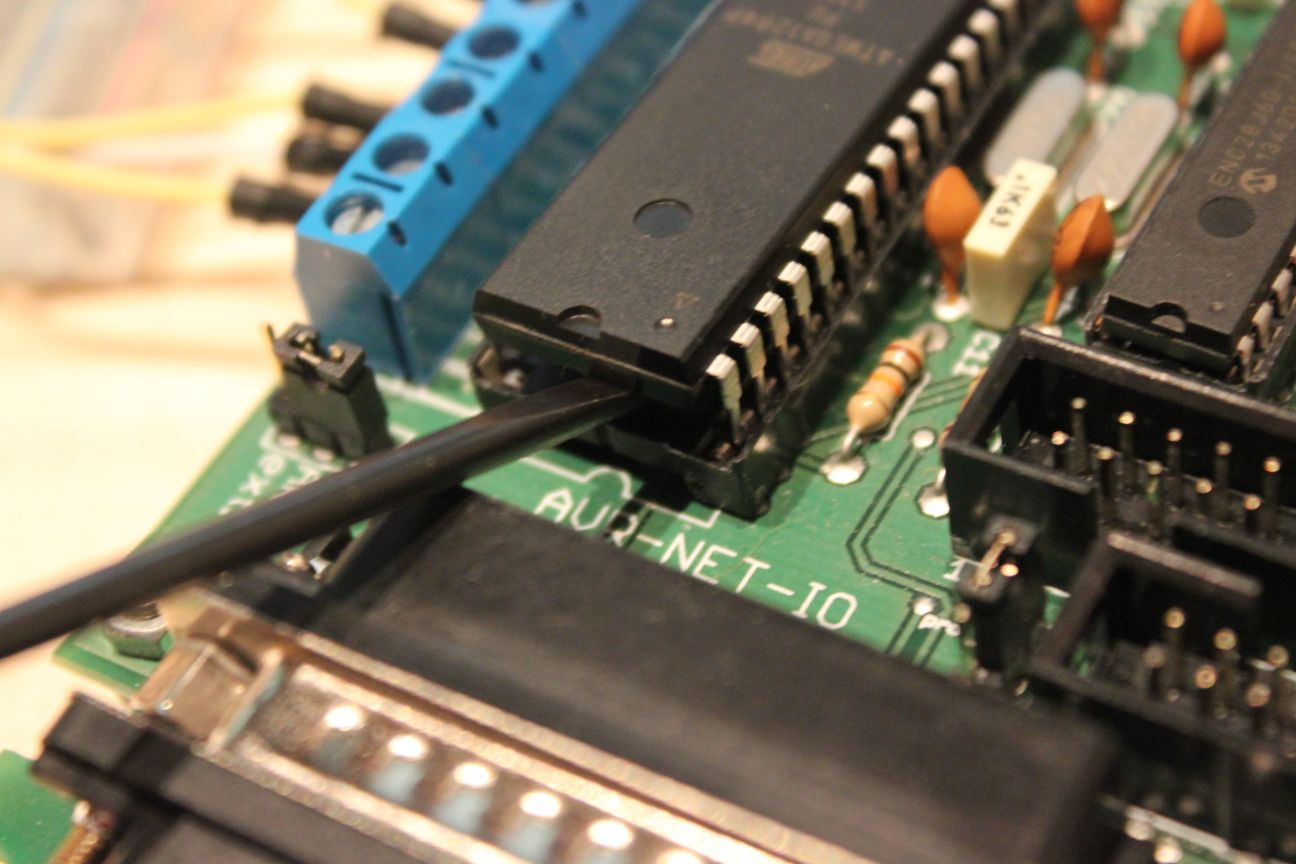
\includegraphics[width=13cm]{content/pictures/Anleitung/tauscheProzessor/1_Hebel.jpg}
\caption{Schraubendreher am Controller}
\label{ausbau1}
\end{figure}

Zum einfachen Lösen kann der Hebel auch von der anderen Seite angesetzt
werden. Anschließend den gelösten Prozessor abziehen.

\begin{figure}[H]
\centering
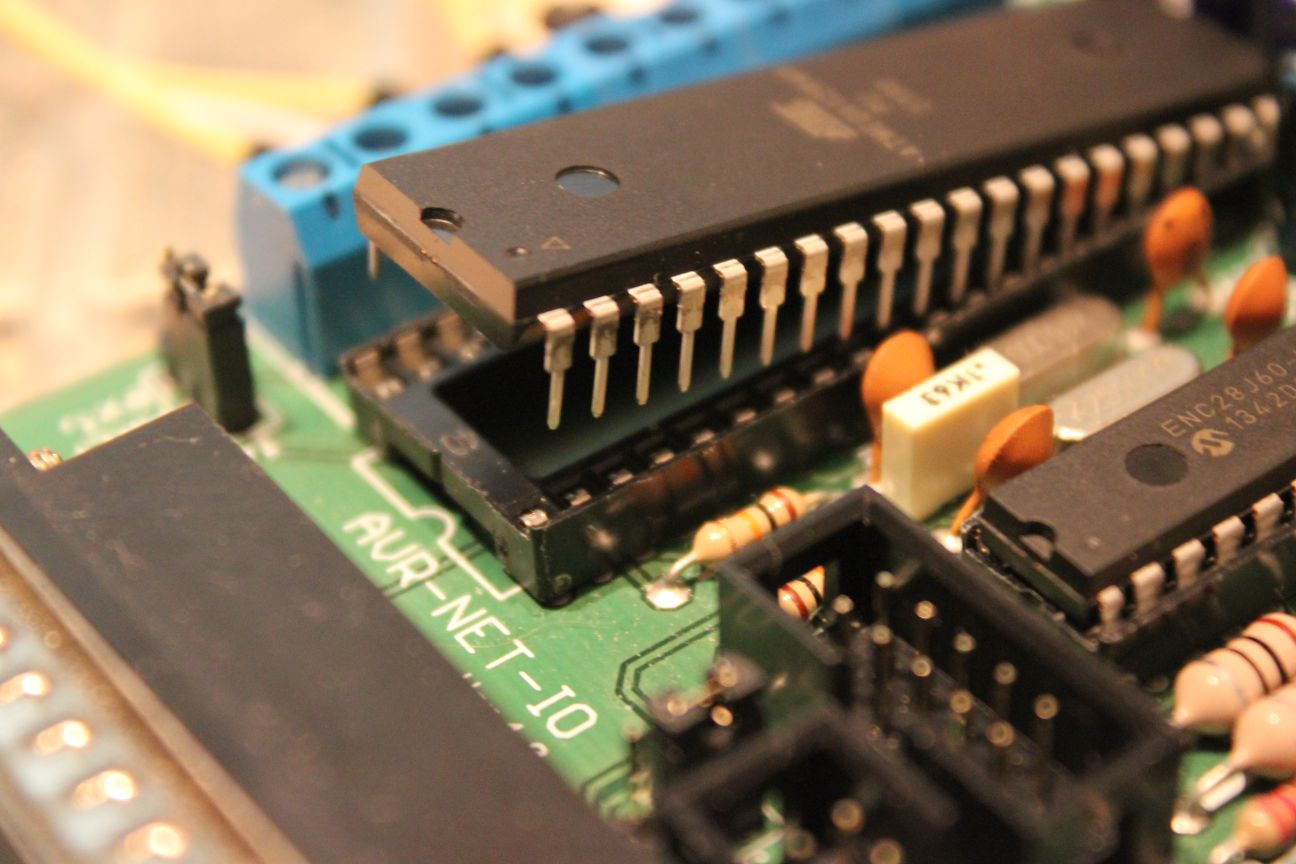
\includegraphics[width=13cm]{content/pictures/Anleitung/tauscheProzessor/2_Geloest.jpg}
\caption{Der gelöste Mikrocontroller}
\label{ausbau2}
\end{figure}

Nachdem der Mikrocontroller entfernt wurde, hat man einen guten Blick auf den
Sockel (Abb. \ref{ausbau3}).

\begin{figure}[H]
\centering
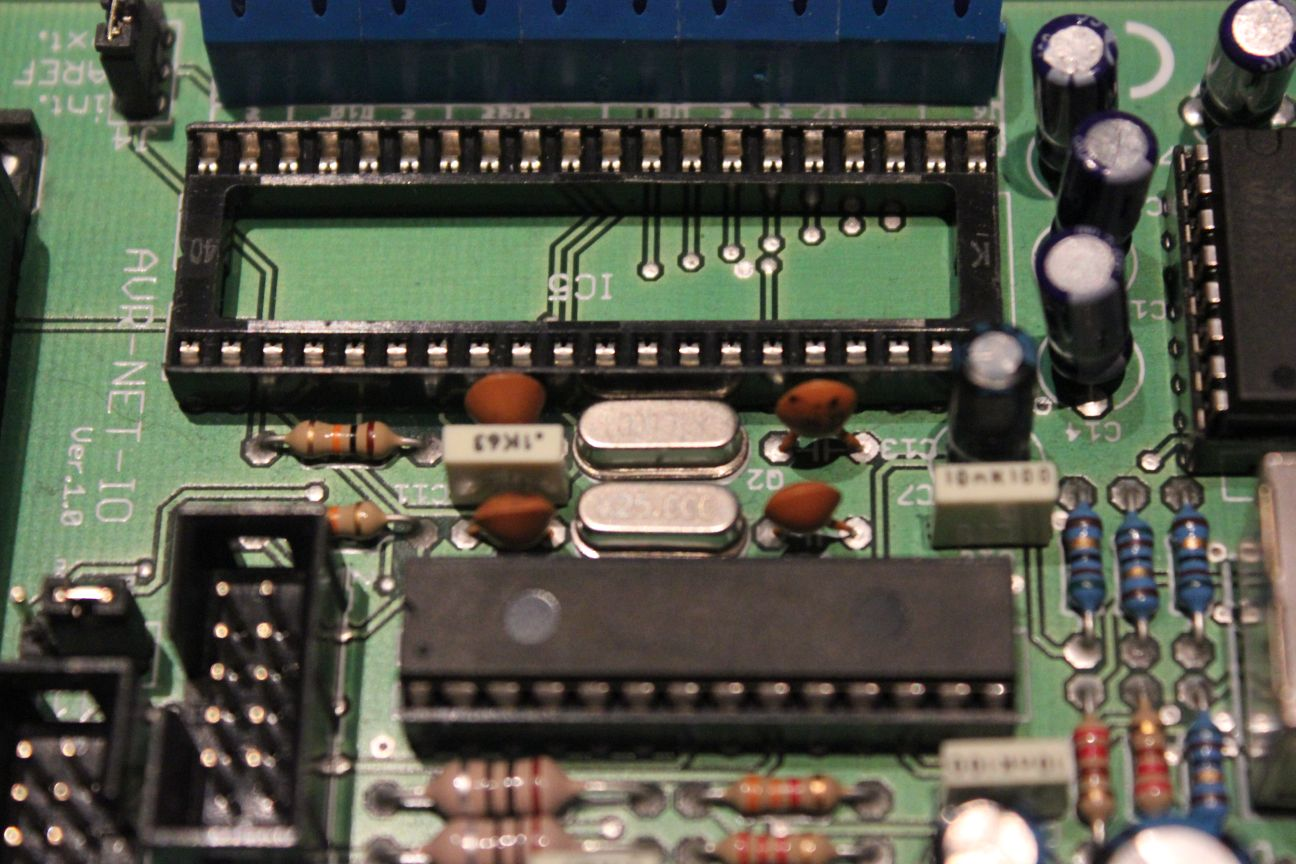
\includegraphics[width=13cm]{content/pictures/Anleitung/tauscheProzessor/3_Sockel.jpg}
\caption{Der Sockel auf dem AVR-Net-IO}
\label{ausbau3}
\end{figure}

Beim Einbau ist unbedingt darauf zu achten, den neuen Mikrocontroller entsprechend
der D-förmigen Einkerbung in den Sockel zu setzen. (Siehe Abbildung \ref{ausbau4})

\begin{figure}[H]
\centering
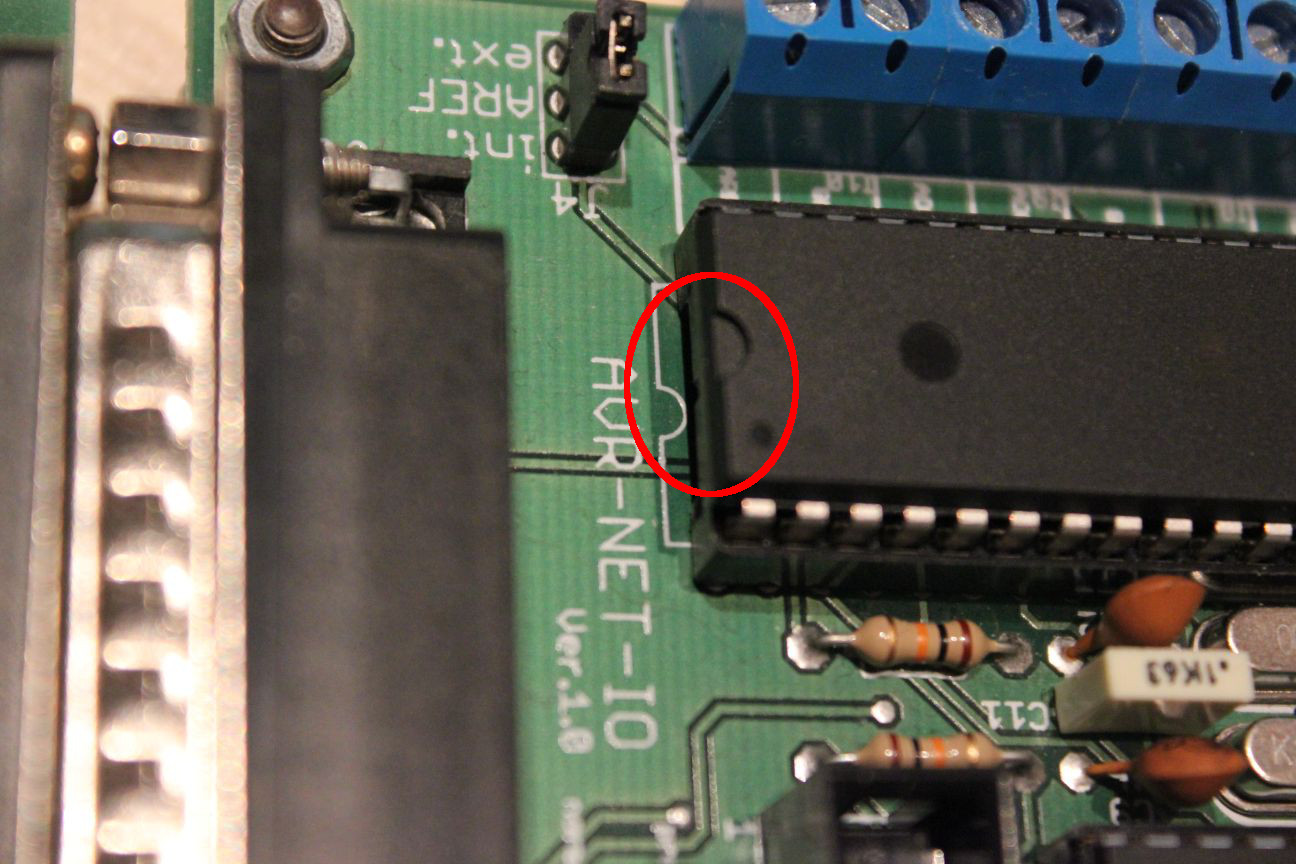
\includegraphics[width=13cm]{content/pictures/Anleitung/tauscheProzessor/4_Markierung.jpg}
\caption{Markierung zum Einbau}
\label{ausbau4}
\end{figure}

\section{ISP-Programmer anschließen}

Der Anschluss des AVRISPmkII Programmers erfolgt über einen 6 Poligen Stecker,
allerdings hat das AVR-Net-IO einen 10 Poligen Stecker. Deswegen wurde hierfür
eigens ein Adapter angefertigt, der das ISP Signal von den 6 Polen des Programmers
auf das AVR-Net-IO bring.

\begin{figure}[htp]
\begin{center}
  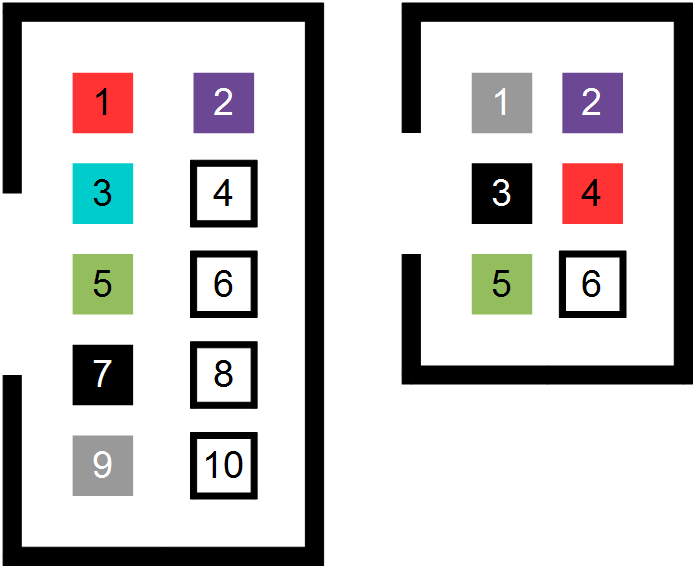
\includegraphics[width=6cm]{content/pictures/Anleitung/ISP-Stecker.png}
  \caption[Schematische Darstellung des ISP Anschlusses]{Schematische Darstellung des ISP Anschlusses (Pin 1 \& 2
  ist auf der Platine markiert)}
  \label{ispanschluss}
\end{center}
\end{figure}

\begin{table}[H]
\centering
\begin{tabular}{|l|l|} \hline
	 \textbf{10-poliger Anschluss} & \textbf{6-poliger Anschluss} \\ \hline
	 1 MOSI & 1 MISO \\ \hline
	 2 VCC & 2 VCC \\ \hline
	 3 - (*) & 3 SCK \\ \hline
	 4,6,8,10 GND & 4 MOSI \\ \hline
	 5 RESET & 5 RESET \\ \hline
	 7 SCK & 6 GND \\ \hline
	 9 MISO &   \\ \hline
\end{tabular}
\caption{Die Pinbelegung für den 6 und 10 poligen Anschluss \cite{mikrocontroller.isp}}
\label{pinbelegung}
\end{table}

\begin{figure}[htp]
\begin{center}
  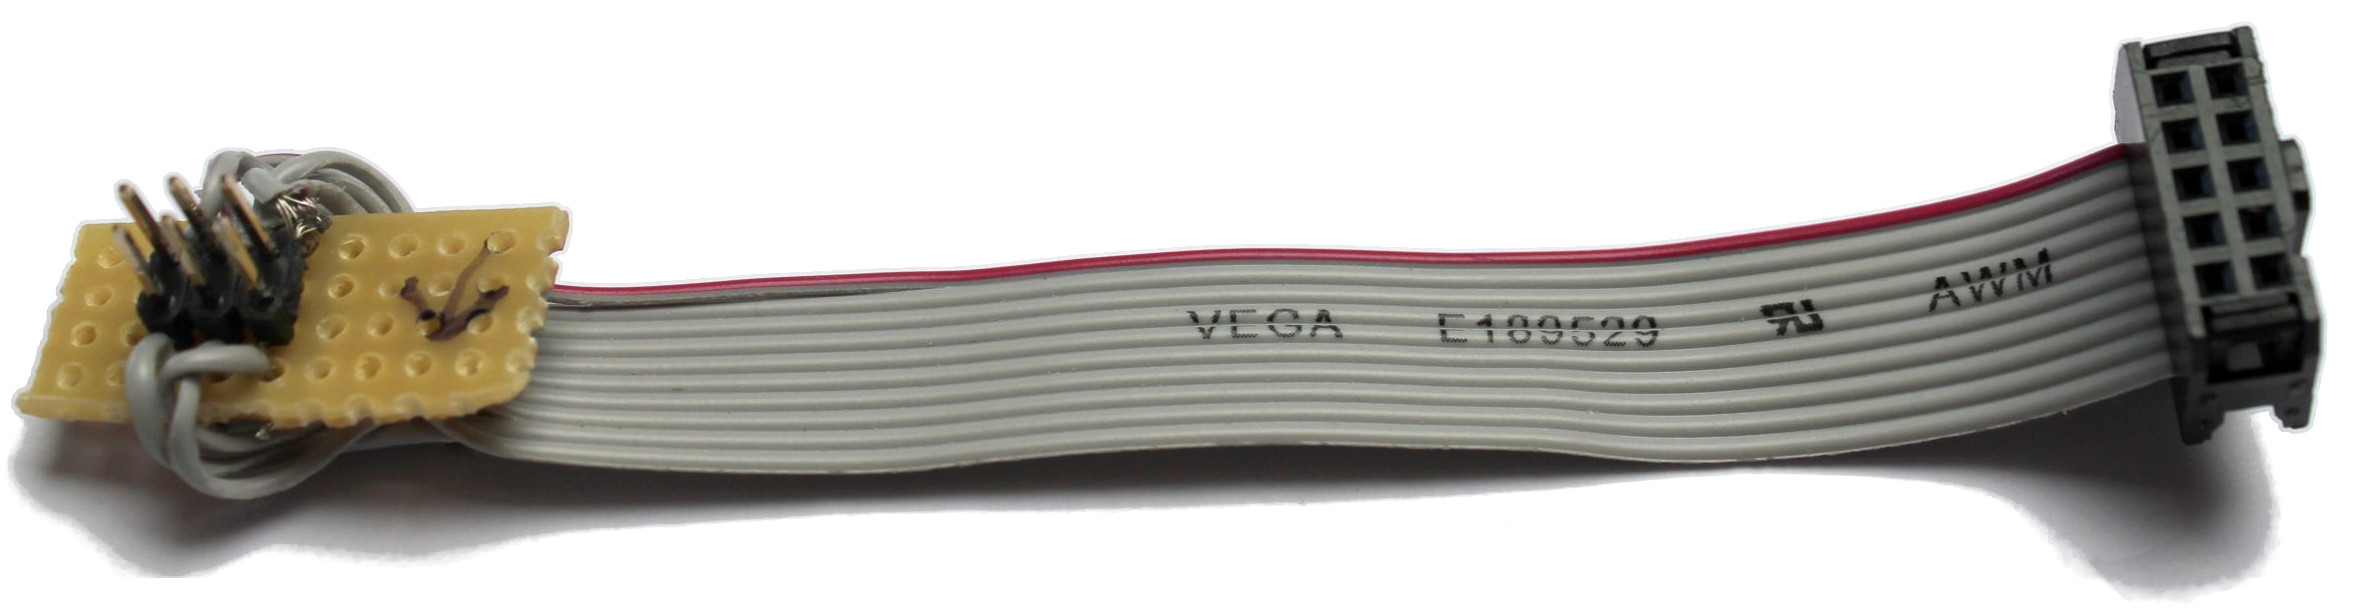
\includegraphics[width=10cm]{content/pictures/Anleitung/adapter.jpg}
  \caption{Der Adapter}
  \label{adapter}
\end{center}
\end{figure}

Mit dem angefertigtem Adapter kann der Debugger anschließend ganz einfach mit
dem Board verbunden werden. Wenn der Mikrocontroller richtig, wie im nächsten Schritt
beschrieben, konfiguriert ist, kann der Programmer auch in Atmel Studio
verwendet werden.

\section{Einrichten eines neuen Mikrocontrollers}
\label{Chapt:Einrichten}

Für einen neuen Chip ist es anfangs notwendig die Fuse-Bits richtig zu setzen,
damit der Chip ordnungsgemäß arbeitet.
Dies ist jedoch im AtmelStudio nicht möglich, da es nicht möglich ist die exakte
Geräte-Signatur auszulesen.
Das Problem liegt darin, dass standardmäßig die Fuses auf den internen
Quarz-Kristall gesetzt sind, und nicht auf den externen Kristall des
AVR-NET-IO Boards.
Beim Versuch die Fuse-Bits zu setzen, erscheint im Atmel Studio die
Fehlermeldung aus Abbildung \ref{Einrichten.error}.

Abhilfe schafft hier die alternative Programmiersoftware AVRDUDE, mit ihr ist
es möglich die Fuse-Bits zu ändern. Unter Linux kann dieser einfach über die
Paketquellen installiert werden, für ein Windows Betriebssystem kann eine
ausführbare Kommandozeilen-Anwendung auf der Projekt-Website heruntergeladen
werden \url{http://savannah.nongnu.org/projects/avrdude}. Zusätzlich muss für
Windows noch libusb-win32 (\url{http://sourceforge.net/projects/libusb-win32/})
vorhanden sein, dass der Programmer mit den gewählten Parametern verwendet werden
kann. Eine ausführliche Anleitung gibt es hier:
\url{http://eliaselectronics.com/using-the-avrispmkii-with-avrdude-on-windows/}

\begin{figure}[H]
\centering
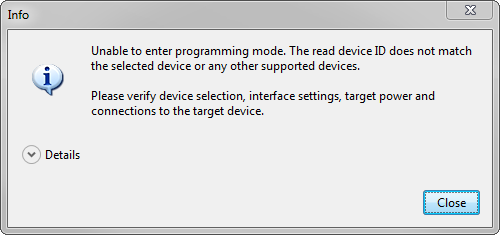
\includegraphics[width=13cm]{content/pictures/Anleitung/neuerProzessor/AnleitungNeuerProzessor2_fehler.png}
\caption{DeviceProgramming}
\label{Einrichten.error}
\end{figure}

Die in folgendem Beispiel angezeigten Befehle sind die von uns verwendeten Fuse
Einstellungen. Für eine genauere Beschreibung, wofür die einzelnen Fuse-Bits
verwendet werden, ist der Abschnitt \ref{chap:Fuse} Fusebits im Kapitel 
"`Hardware"'.

Anschließend kann der Mikrocontroller zusammen mit dem AV-Net-IO und AtmelStudio
programmiert werden. Der verwendete Mikrocontroller wird jetzt richtig erkannt,
da es auch keine Probleme mit der Gerätesignatur gibt.

\begin{table}[H]
\begin{tabular}{| p{.24\textwidth} | p{.76\textwidth} |}
\hline
Auslesen Linux:& sudo avrdude -P usb -p m644p -c avrispmkII  -U lfuse:r:-:h -U hfuse:r:-:h -B 22 \\ \hline
Setzen Linux:& sudo avrdude -P usb -p m644p -c avrispmkII -U lfuse:w:0xFF:m -U hfuse:w:0xD6:m -B 22 \\ \hline
Auslesen Windows:& avrdude.exe -p m644p -c avrispmkII -U lfuse:r:-:h -U hfuse:r:-:h -B 22 \\ \hline 
Setzen Windows:& avrdude.exe -p m644p -c avrispmkII -U lfuse:w:0xFF:m -U hfuse:w:0xD6:m -B 22 \\ \hline
\end{tabular}
\caption{Auslesen und setzen von Fuse-Bits des ATmega644P mit AVRDUDE}
\label{ParameterAvrdude1}
\end{table}

\begin{figure}
\centering
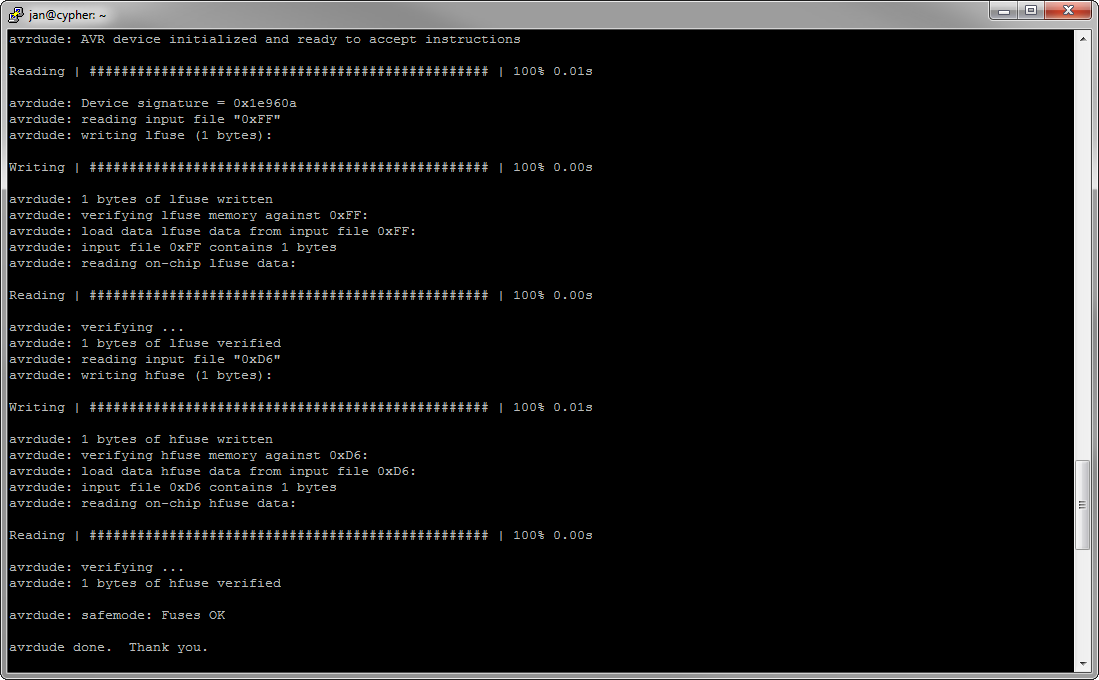
\includegraphics[width=13cm]{content/pictures/Anleitung/neuerProzessor/avrOutput.png}
\caption{AVRDUDE Ausgabe}
\end{figure}

\begin{table}
\begin{tabular}{| p{.35\textwidth} | p{.65\textwidth} |}
\hline
-p partno & This is the only option that is mandatory for every invocation of
avrdude.  It specifies the type of the MCU connected to the programmer. These
are read from the config file.  If avrdude does not know about a part that you
have, simply add it to the config file (be sure and submit a patch back to the
author so that it can be incorporated for the next version). \newline
\textbf{m32 $\Rightarrow$ ATmega32} \newline 
\textbf{m644p $\Rightarrow$ ATmega644P} \newline
\textbf{m1284p $\Rightarrow$ ATmega1284P} \\ \hline
-P port & Use port to identify the device to which the programmer is attached. \textbf{usb für den AVRISP MKII}  \\ \hline 
-c programmer-id & \textbf{avrispmkII für den AVRISP MKII} \\ \hline
-U \hbox{memtype:op:filename:filefmt} &  
The \textrm{memtype} field specifies the memory type to operate on.\newline
\textbf{hfuse} The high fuse byte.\newline
\textbf{lfuse} The low fuse byte.\newline
The \textrm{op} field specifies what operation to perform:\newline
\textbf{r} read device memory and write to the specified file\newline
\textbf{w} read data from the specified file and write to the device memory \newline
The filename field indicates the name of the file to read or write.  The format field is optional and contains the format of the file to read or write. \newline
\textbf{Hier die Bytes die gesetzt werden 0xFF bzw 0xD6} \\ \hline
-B bitclock & Specify the bit clock period for the JTAG interface or the ISP clock \\ \hline
\end{tabular}
\caption{Auszug AVRDUDE Parameter}
\label{parameterAvrdude2}
\end{table}
\newpage

\section{HTML Header Compiler}
\label{chap:benutzerhandbuch.HHC}

Da der HTML Header Compiler in Java entwickelt wurde, muss für die Verwendung die
Java Laufzeitumgebung ab Version 6 installiert sein. Zum Ausführen des Compiler
muss zuerst mit einer Konsole in den Entsprechenden Ordner navigiert werden.
Anschließend kann mit folgendem Befehl die Datei ausgegeben werden. 
\\

\framebox[1.1\width]{java -jar hhc.jar -in <INPUT FOLDER> -out <OUTPUT FILE>} 
\\

Die Angaben in den spitzen Klammern müssen durch den entsprechenden Pfad und
die entsprechende Datei ausgetauscht werden. Standardmäßig optimiert der
HTML Header Compiler die eingegebenen Dateien, falls dies nicht gewünscht ist
gibt es zusätzlich zu den vorgegebenen Optionen weitere Flags
die gesetzt werden können. Hier alle Parameter im Überblick:

\begin{table}[H]
\begin{tabular}{| p{.24\textwidth} | p{.76\textwidth} |}
\hline
-in, -input & Der Eigabepfad mit allen für die Website benötigten Dateien. z.B. \textrm{-in "Webseite"} \\ \hline 
-out, -output & Die Ausgabe Headerdatei z.B. \textrm{-out "Webserver/webpage.h"} \\ \hline
-v, -verbose &  Gibt die ausgegebenen Dateien auf der Konsole aus. \\  
 \hline 
 -n, -newline & Behält die Formatierung für den Zeilenvorschub, Tabulator
 oder Wagenrücklauf in den HTML und JS Dateien (\textbackslash n and
 \textbackslash r \textbackslash t).
 Benötigt dadurch abhängig von der Website mehr Speicher, ermöglicht aber ein
 einfacheres Debuggen von eingebundenem JavaScript Code.  \\ \hline
\end{tabular}
\caption{Parameter des HTML Header Compiler}
\label{parameterHHC}
\end{table}

Um die Entwicklung zu vereinfachen ist es hilfreich, wenn für den Parameteraufruf
des HTML Header Compilers ein einfaches Shell- oder Batch-Script erstellt, das
die Dateien aus dem Ordner für die Website als Headerdatei in den Ordner für den
Webserver schreibt. Falls eine Änderung an der Website vorgenommen wurde, muss
vor dem Programmieren des Mikrocontrollers lediglich der \ac{HHC} ausgeführt
werden.

\begin{figure}[H]
\lstinputlisting[language=sh]{content/code/buildwebpage.sh}
\caption{BuildWebpage.sh für Linux}
\label{output}
\end{figure}

\begin{figure}[H]
\lstinputlisting[language=sh]{content/code/buildwebpage.bat}
\caption{BuildWebpage.bat für Windows}
\label{output}
\end{figure}

\section{Konfiguration des Webservers}

Die Einstellung des Webservers erfolgt über die \textrm{config.h} Datei. In der
\textrm{config.h} Datei, können die verschiedenen Pins der Ports als Ein- oder
Ausgang definiert werden. Dabei gibt es ein paar Eigenheiten zu beachten:
\begin{itemize}
  \item OUTA steht für den A Port, hier ist zu beachten, dass dieser Port die
  Analog zu Digital Wandler beherbergt. Mit aktiviertem Wandler ist es nicht
  möglich, die Pins des Ports funktionierend als Ausgänge zu schalten, da die
  Spannung nicht gehalten wird.
  \item OUTB ist nur mit Vorsicht zu genießen. Hier handelt es sich um den Port,
  der auf dem AVR-Net-IO für die Neztwerkkomunikation genutzt wird. Deswegen
  wird Port B auch nicht standardmäßig definiert.
  \item OUTC dieser Port wird von Pollin standardmäßig für die Ausgänge verwendet
  und ist von uns bereits entsprechend modifiziert. Der gesamte Port wird auf dem
  AVR-NET-IO über den 25Pin D-Sub Stecker geleitet. Wenn der Fuse-Bit für JTag
  geschaltet ist, werden 4 Pins des C Ports für das JTag Interface verwendet.
  \item OUTC Der C Port liegt auf dem AVR-Net-IO auf dem EXT Anschluss und ist
  für erweiterte Peripherie geplant, so kann hier ein Cardreader oder ein
  Erweiterungsboard angeschlossen werden.
\end{itemize}
Weiter kann die gewünschte IP-Adresse eingestellt werden, unter der das Gerät
erreicht werden kann. Wichtig ist hier, dass kein anderes Gerät dieselbe Adresse
im Netzwerk verwendet. Auch kann die Router IP-Adresse und Netzmaske angegeben
werden. Eine weitere wichtige Einstellung ist die verwendete Mac Adresse
des Netzwerkcontrollers. Diese wird über die Variablen MYMAC1-6 definiert.

\section{Debuggen über JTAG}

Der JTAGICEmkII Debugger von Atmel, den wir für unser Projekt gestellt bekommen
haben, unterstützt neben ISP auch JTAG. Allerdings werden für den Anschluss von
JTAG andere Pins benötigt als für den Anschluss eines ISP-Programmers.

\begin{table}
\begin{longtable}{|l|l|l|p{8.8cm}|}\hline 
Pin & Signal & I/O & Description \\ \hline 
1 & TCK & Output & Test Clock, clock signal from JTAGICE mkII to target JTAG port \\ \hline 
2 & GND & - & Ground \\ \hline 
3 & TDO & Input & Test Data Output, data signal from target JTAG port to JTAGICE mkII \\ \hline 
4 & Vtref & Input & Target reference voltage. Also used to power level converter inputs. \\ \hline 
5 & TMS & Output & Test Mode Select, mode select signal from JTAGICE mkII to target JTAG port \\ \hline 
6 & nSRST & Out/-In-put & Open collector output from adapter to the target system reset. This pin is also an input to the adapter so that the reset initiated on the target application board may be reported to the JTAGICE mkII \\ \hline 
7 & - & - & Not connected \\ \hline 
8 & nTRST & NC(Output) & Not connected, reserved for compatibility with other equipment (JTAG port reset) \\ \hline 
9 & TDI & Output & Test Data Input, data signal from JTAGICE mkII to target JTAG port \\ \hline 
10 & GND & - & Ground \\ \hline 
\end{longtable}
\caption{JTAG Connections \cite{JTAGICEmkII.Quick}}
\label{jtag.Connections}
\end{table}

\begin{figure}[htp]
\begin{center}
  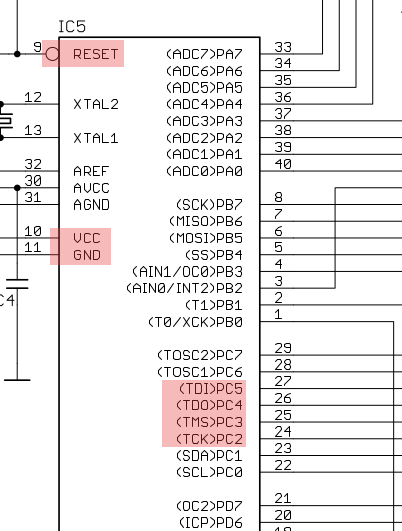
\includegraphics[width=6cm]{content/pictures/jatgPins.png}
  \caption{JTAG Pins}
  \label{jtag.pins}
\end{center}
\end{figure}

Die in Tabelle \ref{jtag.Connections} gezeigten Pins entsprechen der Belegung
der 10 Anschlüssen des JTAGICEmkII. Diese müssen mit den Pins 2-5 des C Ports, dem
Reset Pin, Ground und VCC verbunden werden (Abbildung \ref{jtag.pins}). Die Pins 7 \& 8
des JTAGICEmkII werden nicht mit dem Mikrocontroller verbunden.\\
\\
Damit \ac{JTAG} funktioniert muss der entsprechende JTAG Fuse-Bit gesetzt sein.
Dabei ist zu beachten, dass die Pins 2-5 am Port C des Mikrocontroller nicht für
Ein- oder Ausgaben verwendet werden können, sondern bei aktivierten Fuse-Bit
gesperrt sind. Als weiterer Hinweis ist zu beachten, dass die verwendete
Schnittstelle in den "`Projekt-Einstellungen"' umgestellt werden muss. Nach
korrekter Verbindung, die im Device Manager überprüft werden kann, kann das
Programm auf dem Mikrocontroller debuggt werden.

\section{WinAVR Projekt zu Atmel Studio}

%TODO Beispielexport

\section{Die Website}

Die Webseite ist in 3 Tabs eingeteilt. 

\subsection{Der Status Tab}
Im Status Tab ist die Übersicht der
einzelnen Pins und Ports des Boards. Fährt der Nutzer mit der Maus über die Pins des
Boards, so erscheint auf der rechten Seite des Browser eine Sidebar mit den
detaillierten Informationen zu diesem Pin. Hier können die Pins oder Ports
als Favoriten gespeichert werden. Genauso können Werte und Skripte der einzelnen
Pins oder Ports geändert werden.\\
Ebenfalls kann der Pin mit einem Mausklick gesetzt werden, oder auf der Sidebar in einer 
Checkbox gesetzt werden. Dies kann jedoch nicht mit jedem Pin oder Port gemacht werden, da 
diese Funktion bei manchen nicht möglich sein darf. Diese Pins sind vom System deaktiviert und 
nicht klickbar.
\subsection{Der Favoriten Tab}
Hier werden tabellarisch die ausgewählten Pins oder Ports angezeigt, auch hier
können wieder pinspezifische Modifikationen vorgenommen werden. Löschen der
Favoriten setzt den Pin auf die Standardeinstellungen zurück und ist nicht mehr
in Favoritenliste vorhanden. Pins können wieder über den Status Tab hinzugefügt
werden.

\subsection{Der Einstellungs Tab}
Im Einstellungs-Tab werden die Einstellungen vorgenommen. Hier sind auch die
Informationen über das Board, Version der Webseite und Autoren abrufbar. Die
Import/Export Funktion ermöglicht die Datenbank, in der die Benutzereinstellungen
und Favoriten untergebracht sind, zu exportieren und auf einem anderen System zu
importieren. Die Aktualisierungsrate bestimmt wie schnell sich die Seite
aktualisiert, das ist die einzige Einstellungen die vorgenommen werden kann.

\subsection{Bespiele: Skripte}
Folgend einige Beispielskripte, die nur noch für die passenden Pins und Ports
angepasst werden müssen. Diese Skripte können kopiert und das dafür vorgesehene Fenster
im Webbrowser für die jeweiligen Pins eingefügt werden.

\subsubscetion*{mehrer Lichter blinken}
Hier werden mehrer LED an die Pins D2-D7 angeschlossen\
\begin{figure}[H]
\lstinputlisting[language=js]{content/code/skript_example1.js}
\caption{Beispielskript: Mehrer Lichter blinken lassen}
\label{output}
\end{figure}
Durch den Aufruf dieses Skriptes wird zuerst überprüft ob D2 auf 1
gesetzt ist, ist dies nicht der Fall wird D2 auf 1 gesetzt. Von D3-D7
werden Die Werte abwechselnd 0 und 1 gesetzt. Da dieses Skript dauernd
erneut aufgerufen wird ist somit beim nächsten Aufruf D2 bei 1 und der
Wert wird folglich auf 0 gesetzt. Alle anderen Werte werden auch
geändert. Somit entsteht ein wechseln der Lichter.\newline

\subsubscetion*{Umwandeln in digitale Werte}
Hier werden auch wieder 7 LED verwendet, und ein Sensor angeschlossen
an einen analogen Ports.
\begin{figure}[H]
\lstinputlisting[language=js]{content/code/skript_example2.js}
\caption{Beispielskript: Werte werden in digitale Werte umgewandelt}
\label{output}
\end{figure}
Je nachdem wie sich der Wert von dem Sensor ändert, änderen sich auch die
digitalen Ausgänge zu den LED, ist der gelierferte Wert oberhalb von
869, so wird Anschluss D2 auf 1 gesetzt. Leuchte an D2 leuchtet somit. Da dann
aber alle Abfragen wahr sind werden alle Lichter angeschaltet. sollte dann der
Wert sich unterhalb von 869 befinden dann wird D2 ausgeschalten. Somit ändern
sich immer die Leuchten sobald die neuen Werte überprüft werden.

\subsubscetion*{Lichterlauf}
Bnötigt werden auch hier wieder 7 LED. Angeschlossen an D2 - D7.\\
Mittels diesem Skript werden forlaufend die Lichter nacheinander an und wieder
abgeschalten. Somit entsteht ein Lauf des Aufleuchtens.\newline

\begin{figure}[H]
\lstinputlisting[language=js]{content/code/skript_example3.js}
\caption{Beispielskript: Lichterlauf}
\label{output}
\end{figure}
Zur Erklärung des Skriptes. In einem Case der Switch-Anweisung wird das
vorherige LED ausgeschalten, die nächste LED angeschalten und den Counter
erhöht. Beim nächsten Durchlauf wiederholt sich das immer wieder.


\subsubscetion*{Countdown mit Button}
Für diese Skript wird die 7 Segment Anzeige und ein Button benötigt.\\
Diese Skript lässt die 7 Segment Anzeige nacheinander durchiterieren, sobald
ein button eine bestimmte Zeit gedrückt wird.\newline
\begin{figure}[H]
\lstinputlisting[language=js]{content/code/skript_example4.js}
\caption{Beispielskript: Automatischer Countdown}
\label{output}
\end{figure}
Sobald der Button angeschlossen an A0 gedrückt wird, wird ein Timer ausgelöst.
ist dieser Timer bei 8 und der Button noch gedrückt, wird bei den Anschlüssen
für die Anzeige durchiteriert. Somit ändert sich nur die Anzeige sollte der
Button gedrückt werden. 

\chapter{Rückblick}

\section{Soll/Ist-Vergleich}

\section{Verworfene Varianten}

\section{Eigenbewertung}

\subsection*{Jan-Hendrik Preuß}

\subsection*{Christian Würthner}

\subsection*{Ann-Sophie Dietrich}

\subsection*{Marcel Schlipf}
%Korrekturgelesen: Ann-Sophie Dietrich
\chapter{Ausblick}
In der nächsten Ausbaustufe soll ein Rasberry Pi zwischen den Microcontroller
und die Webseite geschalten werden. Dieses System eröffnet eine Vielzahl
neuer Möglichkeiten, so können von einer Webseite aus mehrere Pollin Net-IO
Boards verwaltet werden und die Favoriten und Skriptfunktionen zentral auf dem
Rasberry Pi gespeichert und von allen Clients verwaltet werden. Auch das Pushen von
Messwerten könnte über dieses System gelöst werden, so muss die Webseite nicht
ständig die Werte pollen.

Für das neue System sind einige Änderungen nötig, diese beschränken sich aber
größtenteils auf den Server, welcher neu eingerichtet werden muss.
%-----------------------------------------------------------------------------------------
\section{Struktur des neuen Systems}
Das neue System besteht folglich aus beliebig vielen Pollin Net-IO Boards, einem
Rasberry Pi und einem oder mehreren Clients. 
\begin{figure}[H]
\centering
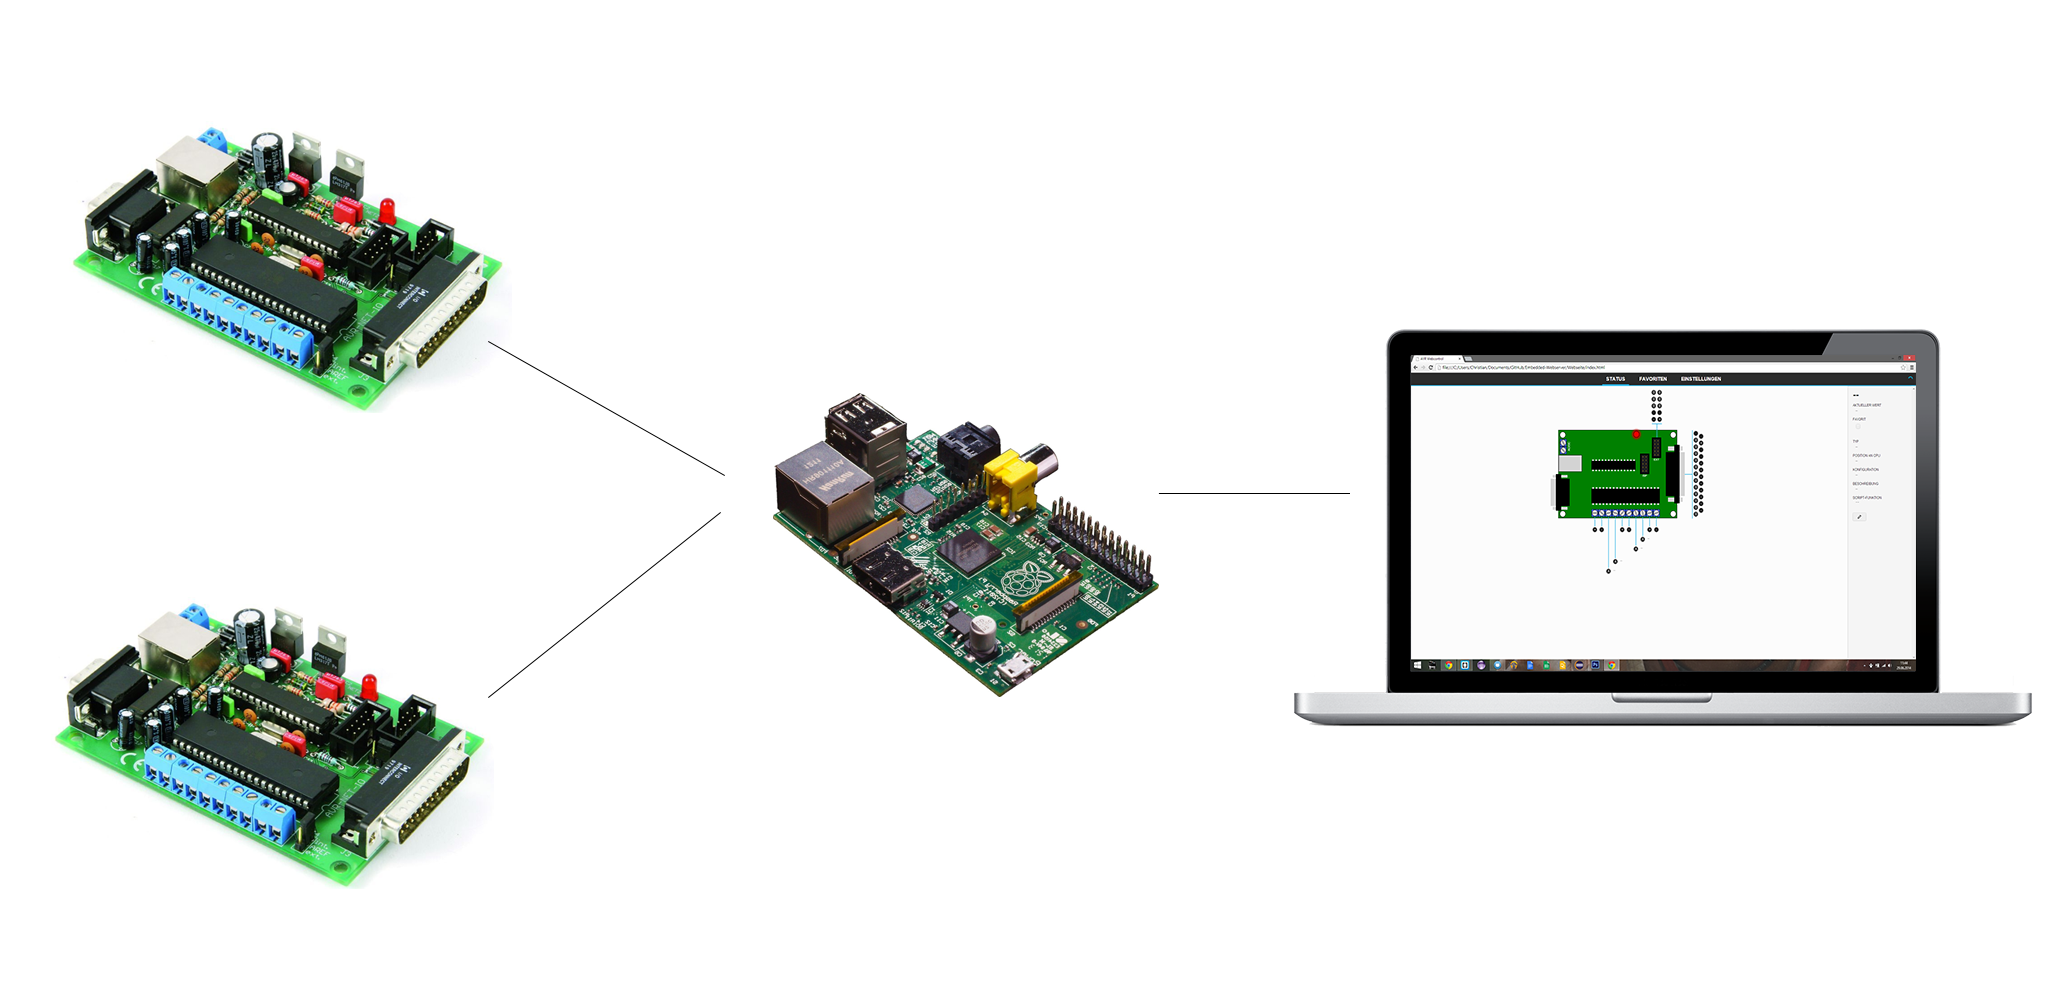
\includegraphics[width=13cm]{content/pictures/neues_system.png}
\caption{Der grobe Aufbau des neues Systems, links zwei Pollin Net-IO Boards,
in der Mitte ein Rasberry Pi und links ein Client}
\label{struktur}
\end{figure}
Die Clients fragen alle Daten, welche in einer kleinen Datenbank
zwischengespeichert werden, von dem zentralen Rasberry Pi ab. So ergeben
sich zwei Teilsysteme: \\
\\
Das erste besteht aus dem Rasberry Pi und den Pollin Net-IO Boards,
welche über die von Pollin bereit gestellte Schnittstelle kommunizieren.
Die Verwendung der bereits vorhandenen Schnittstelle macht es unnötig am
Microcontroller irgendwelche Änderungen vorzunehmen oder eine neue Firmware
flashen zu müssen, was die Usability enorm steigert, da das System auch von
Laien betrieben werden kann. Sobald neue Werte vorliegen sollten die Pollin
Net-IO Boards die Änderungen zum Rasberry Pi pushen, welcher die Werte in einer
kleinen Datenbank zwischenspeichert.Zur Verwendung des bestehenden Protokolls 
muss dieses mit Wireshark analysiert und reverse engineered werden. Hierfür 
kann die Netzwerkkommunikation des Pollin Net-IO Boards mit der mitgeliferten 
PC-Software beobachtet werden.\\
\\
Das zweite System besteht aus dem Rasberry Pi und den Clients. Die Clients
fragen über HTTP beim Server die Webseiten-Dateien und Messwerte ab. Die
Messwerte sollten nicht wie bei der aktuellen Lösung gepollt sondern nur bei
Bedarf mit Hilfe der im Kapitel "`Technischer Hintergrund"' erläuterten HTML5
Server-Sent Events Technik zum Client gepusht werden. Dies reduziert den
unnötigen Netzwerkverkehr. Ein Client kann immer nur ein Pollin Net-IO Board
darstellen, deshalb muss dem Nutzer auf der Webseite die Möglichkeit gegeben
werden, das darzustellende Board auszuwählen. Außerdem muss auf der Webseite die
zu verwendenden Boards (also welche der Rasberry Pi anspricht und den Clients
anbietet) konfiguriert werden können. Ansonsten ist die Webseite ohne große
Änderungen übernehmbar.

%-----------------------------------------------------------------------------------------
\section{Änderungen an der Webseite/Server-Schnittstelle}
\label{aenderung_schnitstelle}
Die Kommunikation zwischen Server und Webseite muss für die neuen Anforderungen
entsprechend erweitert werden. \\
\\
In einem ersten Schritt sollten alle REST-URLs um einen Parameter erweitert
werden, der das Pollin Net-IO Board identifiziert, von dem die Informationen
angefordert werden. Dies ist nötig, da das System über mehrere Boards
verfügen könnte. Der Parameter kann als HTTP-GET Parameter übergeben werden. Als
ID eignet sich z.B. die IP-Adresse des betreffenden Boards oder eine künstliche 
ID in Form einer fortlaufend höheren Zahl. Die aufzurufende URL wäre folglich
z.B. \textrm{/rest/values?id=192.168.2.6}.\\
\\
Danach sollte das aktuell über die POST-Parameter stattfindende
Setzen von Pins ebenfalls über die REST-Schnittstelle gelöst werden. Hierfür
müssen zwei neue URLs eingeführt werden, eine zum Setzen der Pinwerte und eine
zum Setzen des DDRs. Natürlich müssen auch die neuen URLs über den
Parameter zum identifizieren des betroffnen Boards verfügen.\\
\\
Zum Schluss muss noch eine URL bereitgestellt werden um eine Liste aller
verfügbaren Boards abfragen zu können. Zusätzlich muss noch eine URL zum
Hinzufügen eines neuen Boards und eine zum Entfernen eines vorhandenen Boards
angelegt werden.\\
\\
Sobald an der Webseite die Schnitstelle manipuliert wird, ist die Kommunikation
mit dem von uns entwickelten Server nicht mehr möglich. Das System kann nicht
mit HTTP-GET Parametern umgehen. Aus diesem Grund sollte zu Beginn der
Entwicklung ein Testserver aufgesetzt werden. Dieser kann aus einem lokalen
XAMPP-Server bestehen, welcher statt dynamisch Dateien für die
REST-Schnittstelle zu erzeugen über statische Dateien verfügt, welche mit
Testwerten gefüllt sind. So würde z.B. unter \textrm{/rest/pininfo} eine reale
Datei liegen, in der anstatt der Platzhalter feste Werte eingetragen sind. Dies
ermöglicht die Entwicklung der Webseite bzw. dem Ansprechen des Servers ohne
einen funktionsfähigen Rasberry Pi.

%-----------------------------------------------------------------------------------------
\section{Änderungen an der Webseite}
\subsection{Einstellungen}
Die meisten Änderungen der Webseite finden in den JavaScript Dateien statt. Alle
Einstellungen werden mit Hilfe von \textrm{db.js} gespeichert. Aktuell werden
die Einstellungen lokal gespeichert. Dies kann entweder beibehalten werden oder
die Einstellungen können zentral auf dem Rasberry gespeichert werden, was es
ermöglichen würde Favoriten etc. zwischen mehreren Clients zu synchronisieren.
Hierfür müsste nur der Speicherort geändert werden, an dem \textrm{db.js} die
Daten ablegt. Anstatt diese lokal zu speichern müssten sie zum Server geschickt
werden, welcher sie wiederrum an alle anderen Clients weiterleitet.

\subsection{Implementierung der neuen Schnittstelle}
Die neue Schnittstelle zwischen Server und Webseite muss natürlich implementiert
werden. Alle hierfür nötigen Änderungen finden in der \textrm{rest.js} statt.
Neben der Implementierung der Server-Sent Events um neue Messwerte zu
empfangen müssen auch neue Getter und Setter angelegt werden, um z.B. alle
vorhandenen Boards abfragen zu können.\\
\\
Aktuell wird die Funktion \textrm{refreshValues()} dazu verwendet, die Daten
zyklisch nachzuladen. Gestartet wird dieser Vorgang von 
\textrm{startNewRefreshTask()}. Diese Funktionen können in Folge der Umstellung
auf Server-Sent Events komplett gelöscht werden. Wichtig ist hierbei, dass die
Fuktion \textrm{setOnValuesChanged()} und das Attribut
\textrm{onValuesChanged} beibehalten wird. Indem \textrm{onValuesChanged()}
aufgerufen wird, wird \textrm{ui.js} darüber informiert, dass sich die Messwerte
geändert haben, was zur Aktualisierung der Oberfläche führt.

\subsection{Scriptfunktionen}
Aktuell gibt es zwei verschiedene Typen von Skriptfunktionen. Für jeden Pin
lässt sich eine Skriptfunktion zum Erstellen des dargestellten Messwertes
hinterlegen. Diese Skriptfunktionen müssen nicht geändert werden.\\
\\
Zusätzlich gibt es eine Skrtipfunktion die in den Einstellungen festgelegt
werden kann. Sie muss für jedes Board separat verfügbar und anpassbar sein.
Aktuell wird sie auf dem Clientsystem als JavaScript ausgeführt, dass hat zu
Folge das die Skriptfunktion nur so lange funktioniert, wie das Clientsystem
aktiv ist, also die Webseite also angezeigt wird. Diese Skriptfunktion sollte auf dem
Rasberry Pi gespeichert und ausgeführt werden.

\subsection{Auswahl des darzustellenden Boards}
\label{auswahl_board}
Da die Webseite immer nur ein Pollin Net-IO Board darstellen kann, muss dem
Nutzer eine Möglichkeit gegeben werden, eines aus allen verfügbaren auszuwählen.
Hierfür bietet es sich an im \textrm{div} Element mit der ID \textrm{header}
ein \textrm{select} anzubieten (z.B. auf der linken Seite, siehe
Abbildung \ref{select_board}), mit dem das darzustellende Board ausgewählt
werden kann.
Für die Positionierung des Elementes kann das \textrm{div} Element mit der ID
\textrm{loading\_loop} als Vorlage genutzt werden.

\begin{figure}[H]
\centering
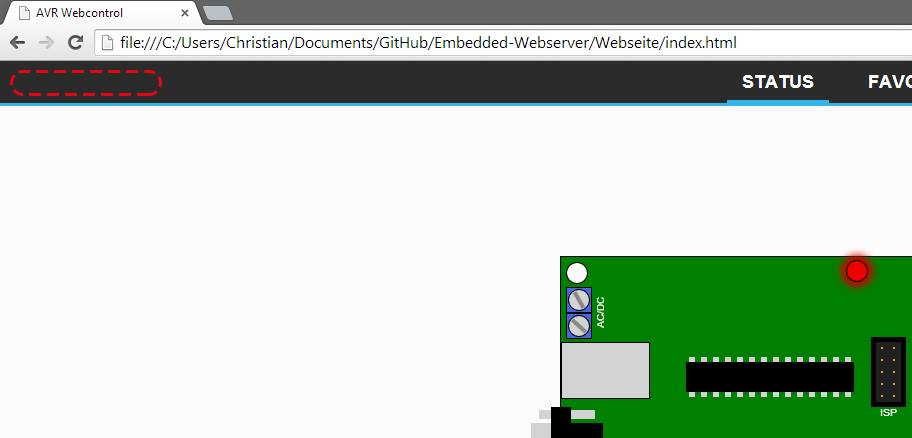
\includegraphics[width=13cm]{content/pictures/select_board.png}
\caption{Vorgeschalgene Position für ein select-Element um die darzustellende
Platine zu wählen}
\label{select_board}
\end{figure}

Beim Einfügen des \textrm{select} Elements in der Header ist zu beachten, dass die
Höhe des Headers nicht verändert werden sollte. Sollte dies dennoch nötig sein,
müssen die Kommentare im CSS-Code beachtet werden, um alle anderen nötigen
Änderungen durchzuführen.

\subsection{Verwaltung der Boards im System}
\label{verwaltung_system}
Im Einstellungs-Tab der Webseite muss eine Möglichkeit ergänzt werden, um die
neue Pollin Net-IO Boards zum System hinzuzufügen und vorhandene zu editieren
oder zu löschen. Für jedes Board sollte eine Sktipfunktion und ein Name
hinterlegbar sein. Der Name ermöglicht es dem Benutzer die Boards leichter
voneinander zu unterscheiden.

%-----------------------------------------------------------------------------------------
\section{Der neue Server}
Beim Server, welcher auf dem Rasberry Pi betrieben werden sollte, gibt es zwei
grundsätzliche Lösungsmöglichkeiten. Zum einen lässt sich der Server als
C/C++/Java-Programm realisieren, das einen Webserver zur Verfügung stellt oder
man realisiert den Server als PHP-Programm auf einem XAMPP-Server.\\
% Satz fängt mit "`zum einen"' an aber es kommt nie ein "`zum anderen"' ?? ..
\\
Bei beiden Alternativen muss der Server mit den einzelnen Pollin Net-IO Boards
kommunizieren, welche Daten über die REST-Schnittstelle bzw. die Server-Sent Events
bereitstellen sowie die Webseite hosten.

%-----------------------------------------------------------------------------------------
\section{Herangehensweise an das Projekt}
\subsection{Einpflegen des Rasberry Pi}
Im ersten Schritt sollte der Rasberry Pi in das bestehende System eingepflegt
werden. Hierfür sollte die Kommunikation zwischen Server und Webseite vorerst so
belassen werden wie sie aktuell ist, inklusive Polling. Der Server muss die
Daten von dem Pollin Net-IO Board empfangen (per Polling oder Pushing) und in
eine kleine Datenbank (oder ein Array etc.) hinterlegen. Bei jeder Abfrage der
Webseite werden die aktuellsten Daten weitergeleitet.\\
\\
Zu beachten ist, dass später die Skripte auf dem Server ausgeführt werden sollen.
Aus diesem Grund würde sich PHP als Programmiersprache anbieten, da PHP-Code,
der als Text vorliegt, direkt mit \textrm{eval()} ausgeführt werden kann.

\subsection{Betreiben mehrer Pollin Net-IO Boards}
Anschließend sollten mehrer Pollin Net-IO Boards betrieben werden können.
Hierfür muss die Server/Webseiten-Schnitstelle entsprechend dem Kapitel
\ref{aenderung_schnitstelle} überarbeitet werden. Die direkte Implementierung
der HTML5 Server-Sent Events ist empfehlenswert. Außerdem muss die Oberfläche
der Webseite um eine Auswahlmöglichkeit für das zu verwendende Board sowie eine
Konfigurationsmöglichkeit für die einzelnen Boards im System erweitert werden
(siehe Kapitel \ref{auswahl_board} und \ref{verwaltung_system}).

\subsection{Verlagern der Skriptfunktionen auf den Server}
Im letzten Schritt sollten die Skriptfunktionen, die nach jedem Neuladen der
Werte ausgeführt wird (aktuell im Settings-Tab einstellbar), auf dem Server
gespeichert und ausgeführt werden. Die Skriptfunktionen müssen natürlich von der
Webseite aus für jedes Board einzeln anpassbar sein. 
Wenn die Serverstruktur auf Basis des
XAMPP-Servers gewählt wurde, bietet sich PHP als Skriptsprache an, da der Code
nach dem Empfang neuer Werte direkt mit \textrm{eval()} ausgeführt werden kann.
Wichitg ist hierbei, dass über einfache Getter und Setter Funktionen der Zugriff
auf alle aktuellen Messwerte möglich ist und die Skriptfunktion auch Pins von
Boards sowie deren DDR manipulieren kann.

\chapter{Fazit}

Die Welt der Mikrocontroller steckt voller Möglichkeiten ist aber auch mit
einigen Schwierigkeiten behaftet. Anders als beim arbeiten mit Computern bei
denen der Speicherplatz für einfache Programme schier unbegrenzt ist kommt es bei
den Mikrocontroller auf jedes Byte an. So bestand in unserem Projekt nicht nur
die Schwierigkeit darin den Server mit weiteren Funktionen auszustatten sondern
auch bei der Programmierung möglichst auf Effizienz zu achten und den
bestehenden Webserver von nicht benötigten Funktionen zu befreien. Als eine
weitere Herausforderung bei Mikrocontrollern kommt noch die ganze elektronische
Seite hinzu. Als Informatiker haben wir durch das Studium kaum Berührung mit
diesem Thema gehabt und mussten uns vielerorts in die Themaktik einarbeiten.
Doch hat sich das Projekt als handhabbarer erwiesen als anfangs gedacht. Die
Hauptaufgaben bestanden hier im beschaffen von Bauteilen, dem
erstellen von Platinen zum Testen der Funktionen oder dem Programmieren und
Debuggen des Mikrocontrollers.




% Schalgwortverzeichnis (Index)
%\printindex

% Literaturverzeichnis
\singlespacing
\bibliographystyle{alphadin}
\bibliography{bibtex}

% Eidesstattliche Erklärung
%\include{content/affirmation}

\appendix
% Hier können Anhaenge angefuegt werden

\end{document}      